\appendix

%真实的需要的附录部分

\begin{figure}[htbp]
\centering
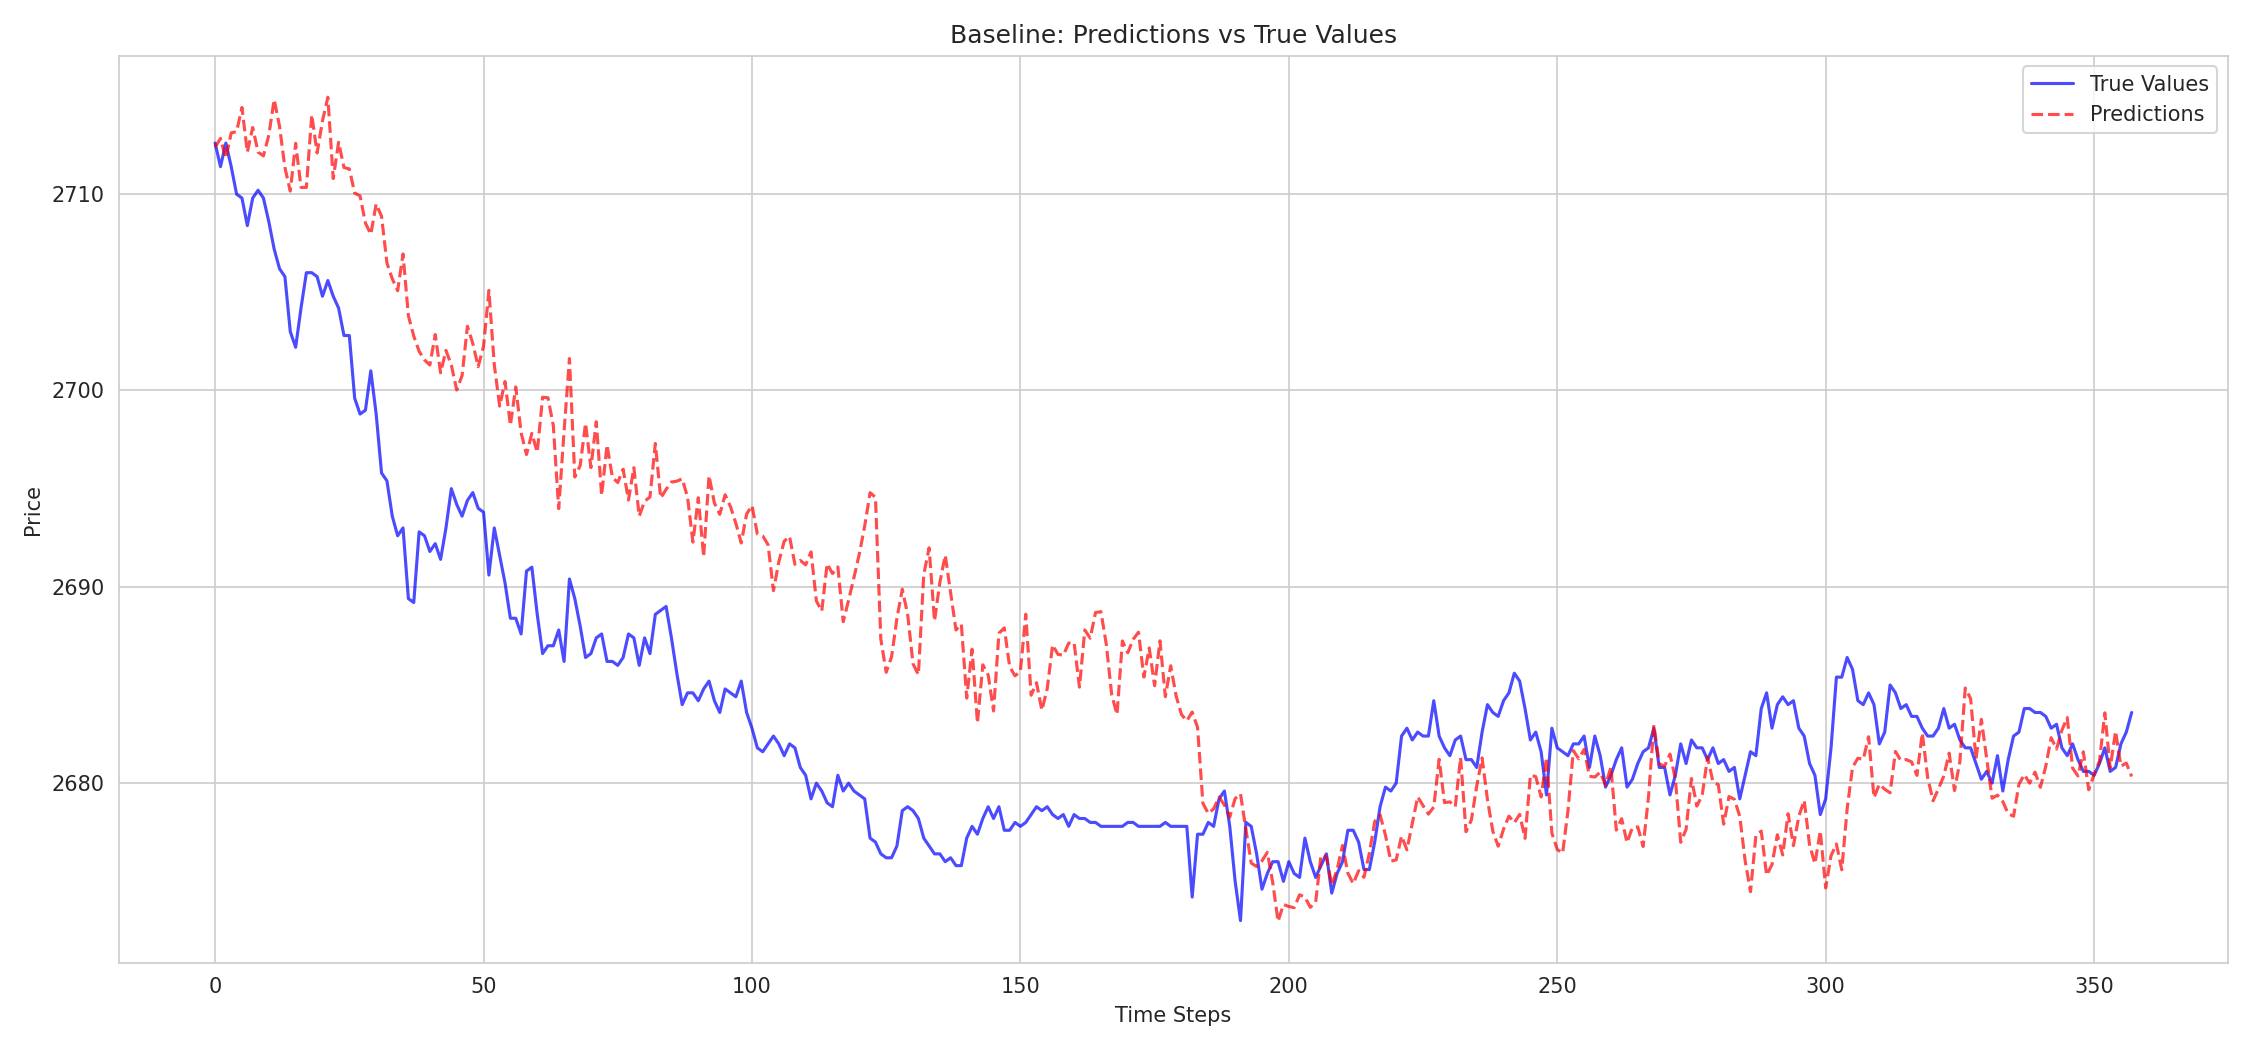
\includegraphics[width=0.85\textwidth]{TongjiThesis-master/figures/chap6/IH_seg7_exp0_baseline_predictions.png}
\caption{Baseline模型在上证50股指上的价格预测表现}
\label{fig:IH9999exp0baselinepredictions}
\end{figure}


\begin{figure}[htbp]
\centering
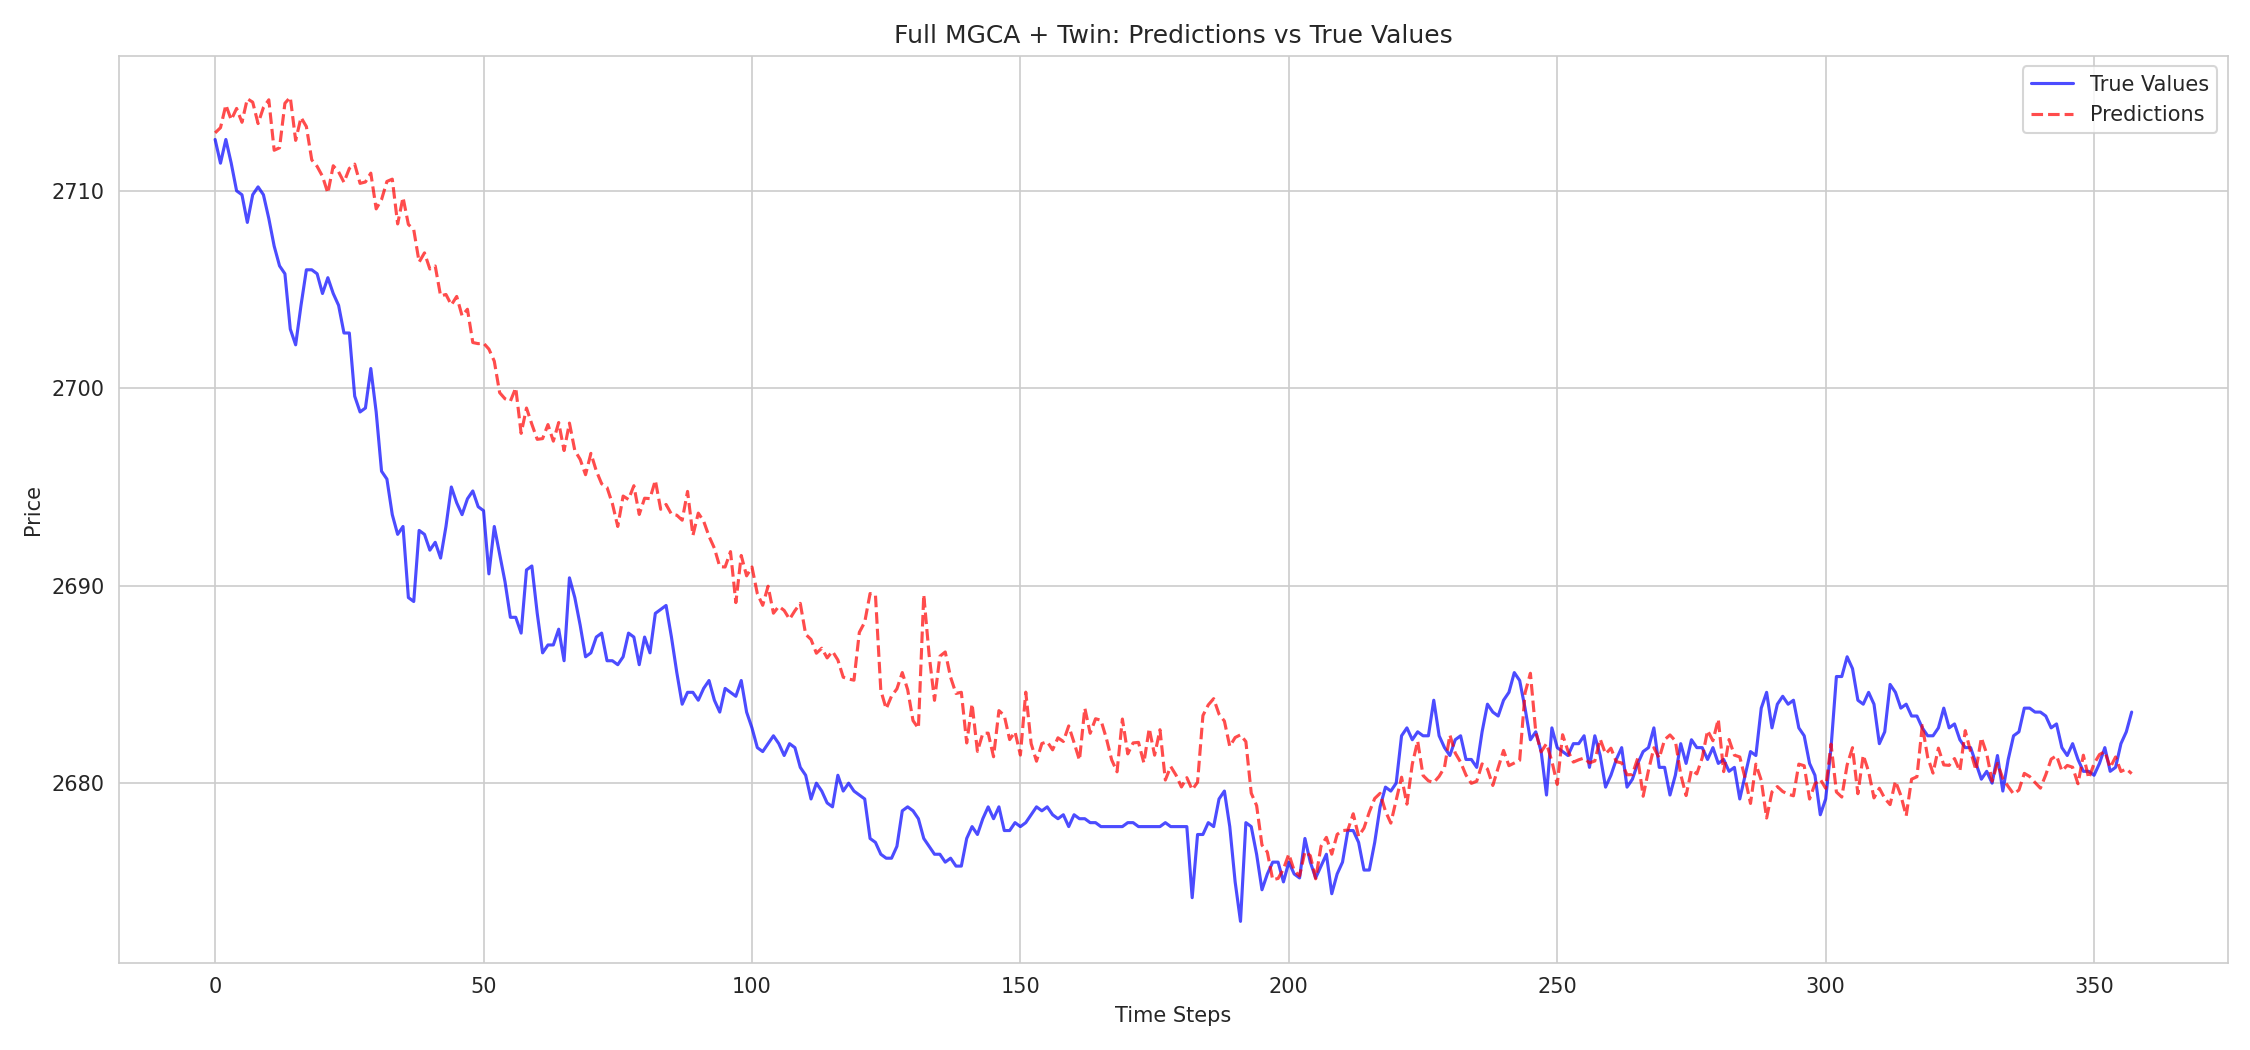
\includegraphics[width=0.85\textwidth]{TongjiThesis-master/figures/chap6/IH_seg7_exp7_full_mgca_twin_predictions.png}
\caption{孪生对抗框架在上证50股指上的价格预测表现}
\label{fig:IH9999exp7twinpredictions}
\end{figure}

上证50股指期货是孪生对抗框架表现最优异的品种，也是金融期货类的代表性品种。上证50股指包含12个时间段，每段2,500个数据点，总计30,000个数据点。该品种的价格受到股市整体走势、宏观经济数据、政策变化、市场情绪等多种因素的综合影响，价格波动较为剧烈，但相比有色金属仍处于可预测的范围内。上证50股指是孪生对抗框架表现最为卓越的案例之一。从图\ref{fig:IH9999exp0baselinepredictions}和图\ref{fig:IH9999exp7twinpredictions}的对比可以看出，孪生对抗的MAPE为0.0291，相比Baseline的0.0360改善了19.29\%。更令人瞩目的是，该实验实现了21,820.44元的成本改善，充分展示了框架在金融期货交易中的实际价值。

预测曲线显示，孪生对抗在整个时间序列上都保持了与真实价格的高度一致性，特别是在价格波动较大的区域，其预测曲线能够准确跟随真实价格的变化轨迹，而Baseline的预测则显得相对滞后或过度平滑。这种预测质量的提升，结合优秀的成交量预测能力，使得孪生对抗在VWAP执行中能够实现更优的订单分配，从而显著降低交易成本。在上证50股指的12个时间段中，平均成本节省达到15,173元，盈利胜率75.0\%，相比Baseline实现了7,063元的成本改善。

\begin{figure}[htbp]
\centering
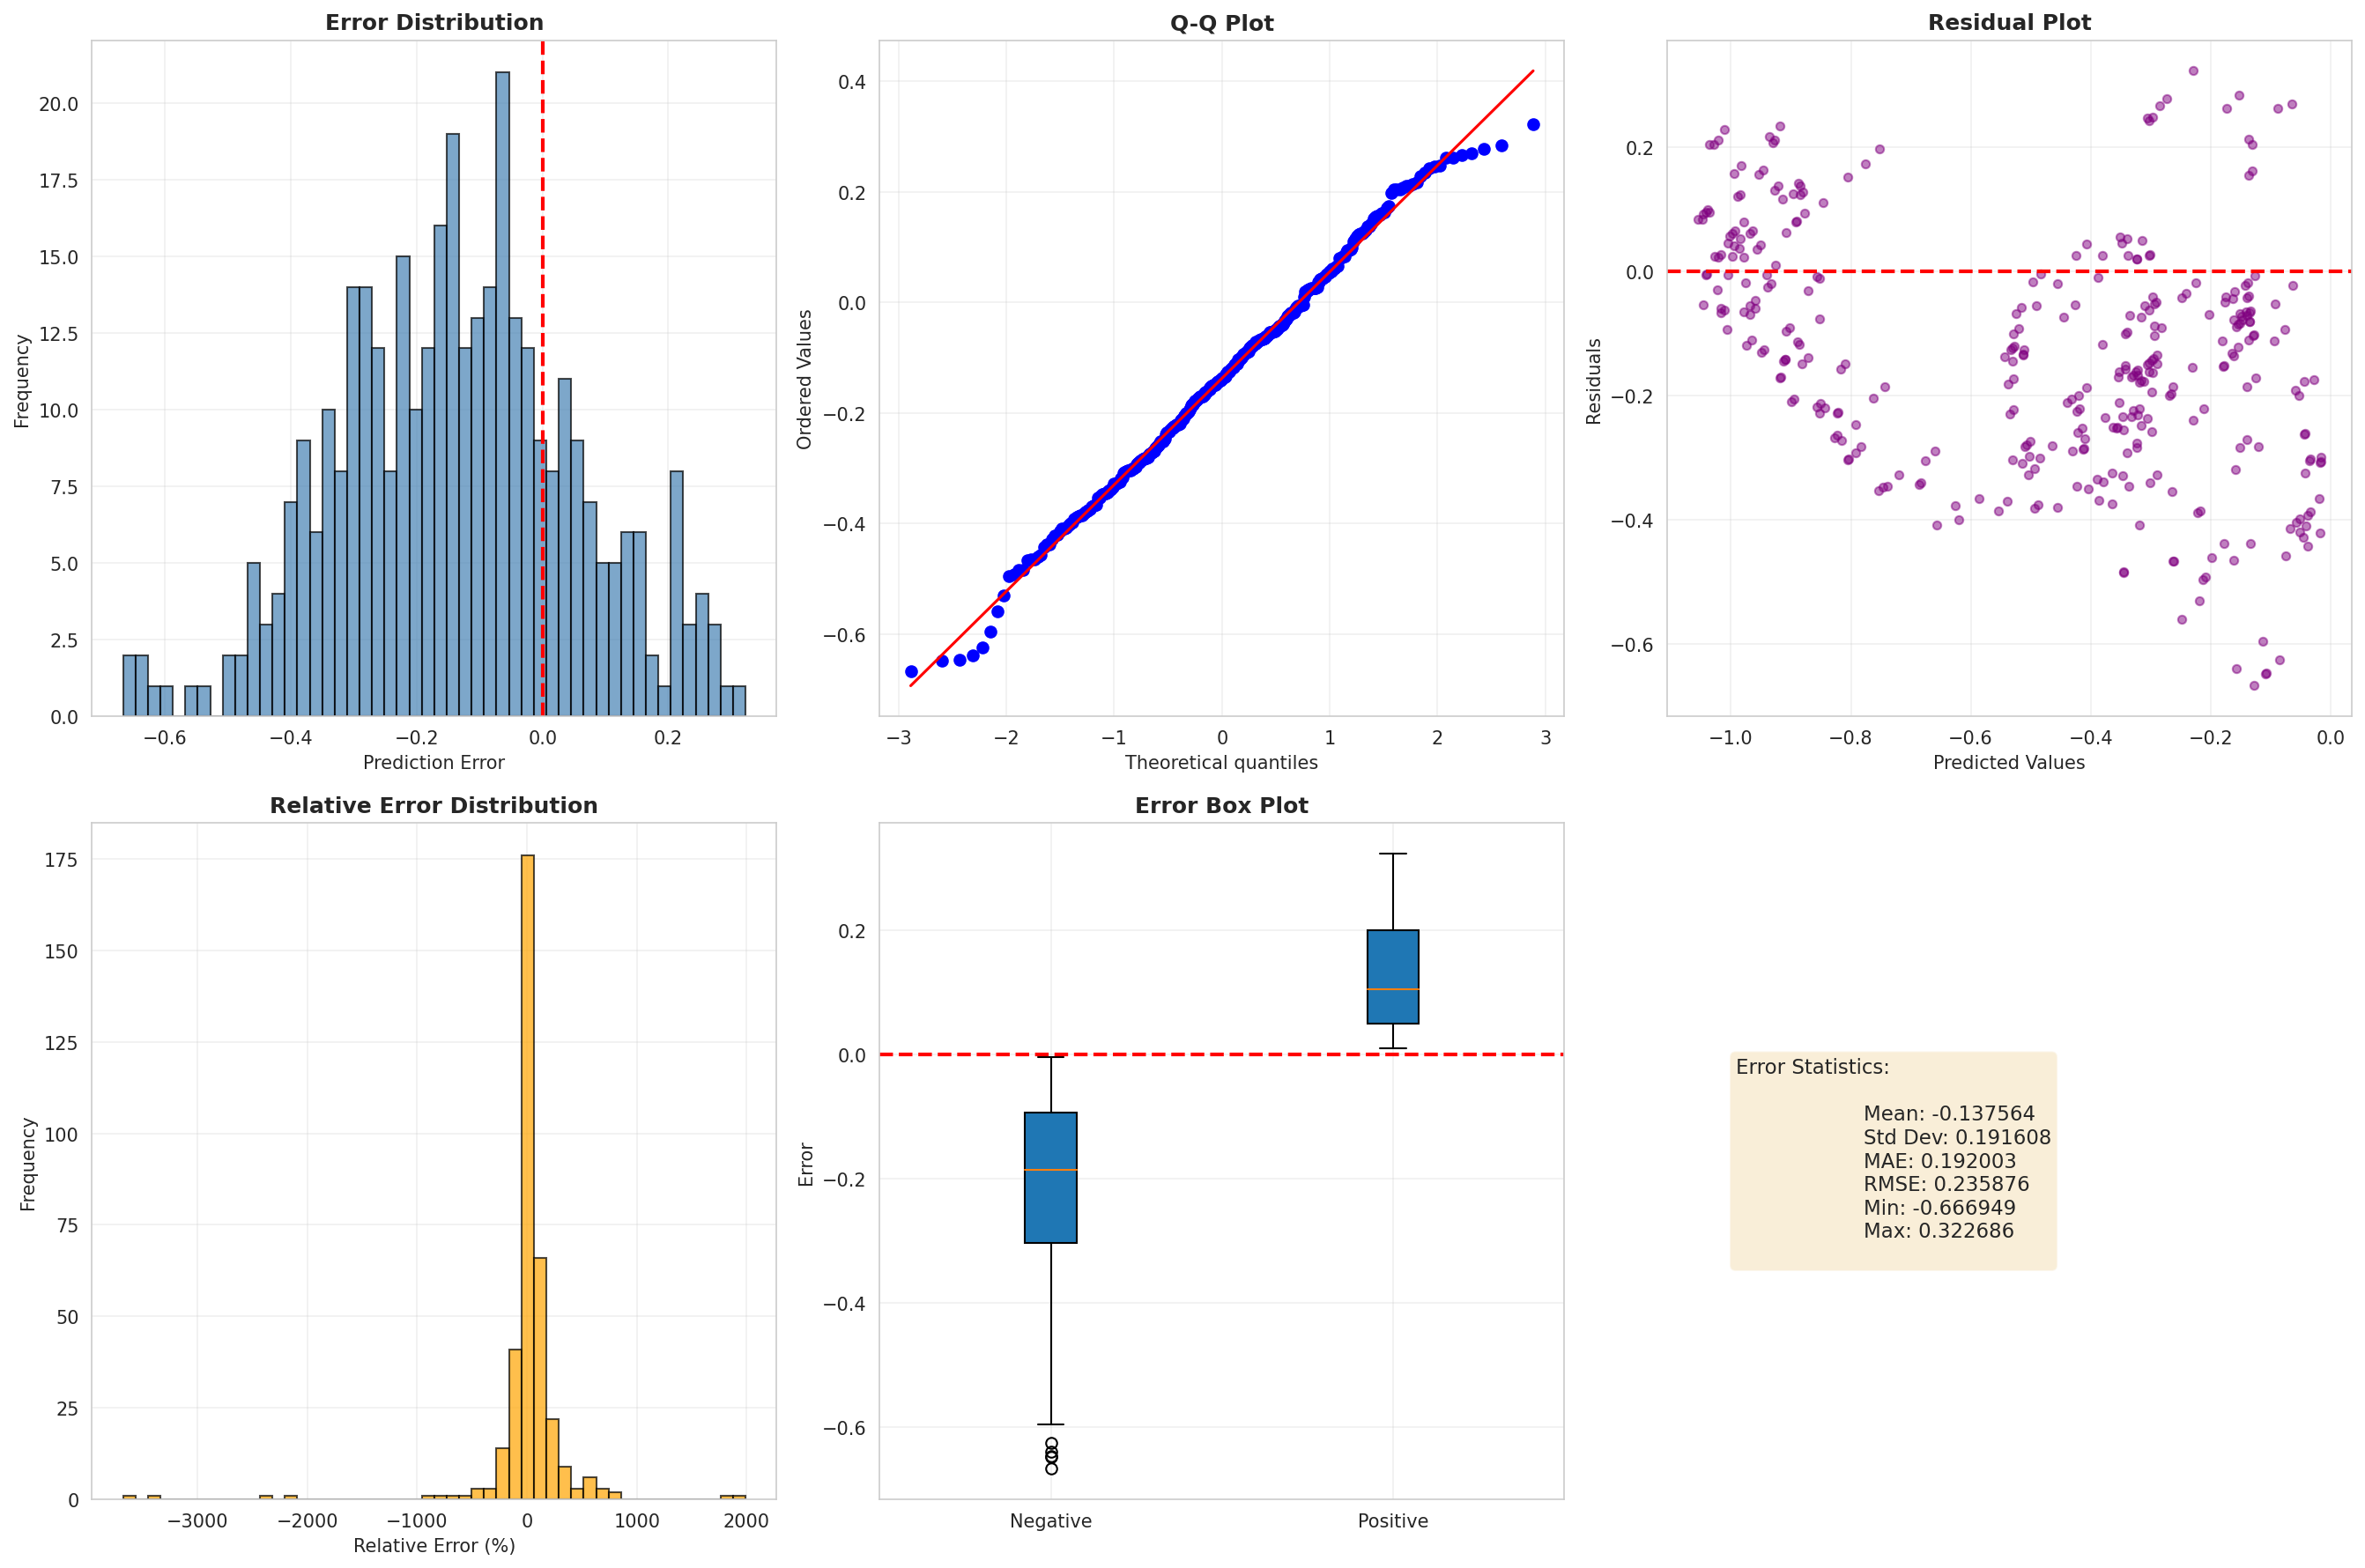
\includegraphics[width=0.85\textwidth]{TongjiThesis-master/figures/chap6/IH_seg1_exp7_full_mgca_twin_error_analysis.png}
\caption{孪生对抗框架在上证50股指（IH9999数据集）上的误差分布}
\label{fig:IH9999exp7twinerroranaly}
\end{figure}

上证50股指的误差分布\ref{fig:IH9999exp7twinerroranaly}同样呈现良好的统计特征。误差偏度为0.156，接近0，表明预测不存在系统性高估或低估的倾向。误差峰度为3.42，略高于正态分布的3.0，表明极端误差的出现频率略高于正态分布的预期，这是股指期货的典型特征，因为股市中偶尔会出现由重大事件驱动的剧烈波动。Q-Q图显示误差分布在中心区域与正态分布高度吻合，仅在尾部存在轻微的厚尾现象，这与金融时间序列的尖峰厚尾特征一致。

\begin{figure}[htbp]
\centering
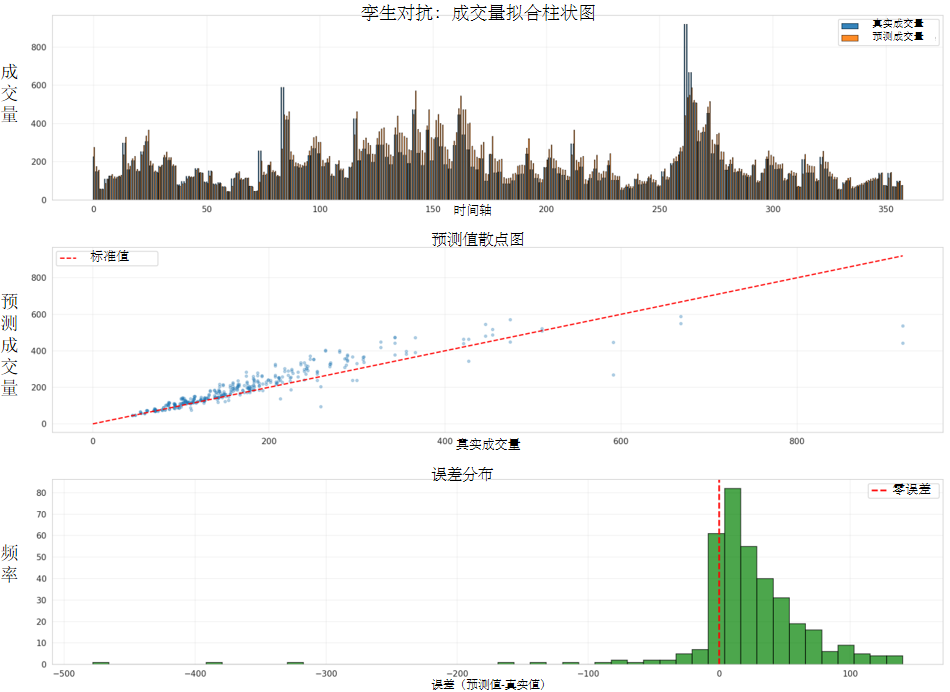
\includegraphics[width=0.85\textwidth]{TongjiThesis-master/figures/chap6/TWIN_distribution_volume_cn.png}
\caption{孪生对抗框架在上证50股指（IH9999数据集）上的成交量预测对比}
\label{fig:IH9999exp7twinvolumecomp}
\end{figure}

上证50股指的成交量预测\ref{fig:IH9999exp7twinvolumecomp}同样表现出色。从图可以看出，预测成交量与真实成交量的柱状图高度重叠，成交量MAPE为25.76\%，虽然略高于黄金的7.99\%，但考虑到股指期货成交量的高波动性和复杂性，这一表现已经相当优秀。股指期货的成交量具有明显的日内模式（开盘和收盘时段放量）和事件驱动特征（重要数据发布、政策公告等），孪生对抗的多生成器架构能够更好地捕捉这些复杂模式。

%真实的需要的附录部分


% \section{Details of Methodology}
% \label{sec:appendix Methodology}
% \subsection{Multi-Source Feature Encoder}\label{sec:appendix multi_source}
% Each $Encoder_m$ utilizes a Transformer encoder as its backbone network. For the input sequence $X_{G_m}\in \mathbb{R}^{T \times D_{G_{m}}}$ of the $m$-th feature group (where $T$ is the sequence length and $D_{G_{m}}$ is the dimension of the $m$-th feature group), the input features are projected onto the model's latent dimension $d_{model}$ via a linear layer:
% \begin{equation}
% \mathbf{x}_{G_{m}, t}^{\prime}=\mathbf{x}_{G_{m}, t} \mathbf{W}_{\text {input }, m}+\mathbf{b}_{\text {input }, m},
% \end{equation}
% where $\mathbf{x}_{G_{m}, t}^{\prime}$ is the input vector of the $m$-th feature group at time step $t$. Subsequently, to encode the temporal order information of elements in the sequence within the model, position encoding $PE$ in the form of sine and cosine functions is introduced:
% \begin{equation}
%     \begin{aligned}
%         \mathrm{PE}_{(pos, 2 i)}&=\sin \left(\frac{pos}{10000^{2 i / d_{\text {model }}}}\right), \\ \mathrm{PE}_{(pos, 2i+1)}&=\cos \left(\frac{pos}{10000^{2i/d_{\text{model}}}}\right),
%     \end{aligned}
% \end{equation}
% where $pos$ denotes the position in the sequence, and $2i$ and $2i+1$ denote the dimension indices, enabling the model to understand the relative and absolute positional relationships between data points in the sequence. Ultimately, each encoder $Encoder_m$ outputs its corresponding feature group's latent representation $h_{G_{m}} \in \mathbb{R}^{T \times d_{\text {model}}}$.

% \subsection{Downstream Task Fine-tuning}\label{sec:appendix downstream_tasks}
% \textbf{Regression Prediction}.
% For prediction tasks involving continuous values such as stock prices and index changes, a regression predictor $Predictor$ is introduced. This predictor takes the feature vector from the last time step of the joint latent representation $h_{combined}$ output by the Multi-Source Feature Encoder as input, further processes it through a Transformer backbone network, and finally outputs the predicted value $\hat{y}_{\text {regress }}$ through a linear layer:
% \begin{equation}
% \hat{y}_{\text {regress }}=\operatorname{Predictor}\left(h_{\text {combined }}[:,-1,:]\right)
% \end{equation}
% During training, MSE is used as the loss function to minimize the difference between the predicted value and the true target $y_{\text{true}}$:
% \begin{equation}
% \mathcal{L}_{\text {regression }}=\left\|\hat{y}_{\text {regress }}-y_{\text {true }}\right\|_{2}^{2}
% \end{equation}

% \textbf{Classification Prediction}
% For the classification task of predicting the future trend of financial assets (e.g., whether the price will rise or fall the next day), a classifier $Classifier$ is used. The classifier also takes the feature vector from the last time step of the joint latent representation output by the Multi-Source Feature Encoder as input, processes it through a Transformer backbone network, and finally outputs the logits for each category.
% \begin{equation}
% \text { Logits }=\text { Classifier }\left(h_{\text {combined }}[:,-1,:]\right)
% \end{equation}
% For multi-class classification tasks, the cross-entropy loss function is used for optimization:
% \begin{equation}
% \mathcal{L}_{\text {class}}=-\sum_{k=1}^{N_{c}} y_{\text {true }, k} \cdot \log (\operatorname{Softmax}(\operatorname{Logits})_{k})
% \end{equation}
% where $N_{c}$ is the number of categories, and $y_{\text{true }, k}$ is the One-Hot encoding of the true category.

% \textbf{Investment Decision}.
% This task mode is specifically designed for quantitative financial investment decisions, aiming to optimize the expected return based on predicted actions directly. Unlike traditional classification tasks that merely predict trends, the goal of this model is to learn decision strategies that maximize actual investment returns. 

% The $Classifier$ still outputs Logits for different investment actions (e.g., going long (buying), going short (selling), holding). These Logits are converted via the Softmax Function into predicted probabilities $p(a|x)$, representing the probability of taking action $a$ on a given input $x$.

% For the investment task, the $y_{\text{true}}$ represents the actual price change. The potential return $r(a)$ for each action $a$ is defined. For a 3-class investment task, the actions are typically: Class 0 (Price Down), Class 1 (Price Stable), Class 2 (Price Up). The corresponding action coefficients $\text{action\_coefficients} = [-1.0, 0.0, 1.0]$ are used to define the return for each action given the actual price change:
% \begin{equation}
% r(a) = y_{\text {price\_change }} \cdot \text { action\_coefficients }[a]
% \end{equation}
% The training objective of the model is to maximize the expected reward across all samples in a batch, which is equivalent to minimizing the negative expected reward loss:
% \begin{equation}
% \mathcal{L}_{\text {investment }}=-\mathbb{E}_{x}\left[\sum_{a} p(a \mid x) \cdot r(a)\right]
% \end{equation}
% This customized loss function enables the model to directly learn the features and patterns that are most economically meaningful for actual investment decisions, thereby achieving optimal strategies and returns in both simulated and real market environments.

% \section{Data and Benchmark}
% \label{sec:appendix Data_Benchmark}
% \subsection{Dataset and Backtesting Period}\label{sec:appendix dataset}
% The data utilized in the experiments was sourced from authoritative financial databases such as Wind and Oriental Fortune, covering daily market data from January 2005 to June 2025. This comprehensive dataset includes asset prices, trading volumes, technical indicators, and fundamental data. During the preprocessing phase, missing values were imputed, data were standardized, and logarithmic returns were calculated across all data dimensions.

% \begin{itemize}
% \item The chosen period encompasses a variety of market scenarios, including the impact of pandemics, geopolitical conflicts, and macroeconomic cyclical reversals. This diverse coverage is crucial for demonstrating the strategy's robustness in complex and non-stationary markets. Furthermore, the phased data partitioning strictly avoids future data leakage, ensuring an objective assessment of the model's performance.
% \item Features incorporate multi-level information, including raw technical indicators, rolling window statistics, and cross-sectional normalization. Target variables are processed according to their task type, appearing as return regressions, up/down labels, or optimal weight guidance signals. The data is organized in a pandas \textit{DataFrame}, compatible with PyTorch model input interfaces, and processed into aligned, batched inputs via a unified data loader. Overall, this experimental design comprehensively covers potential strategy combinations in real-world financial scenarios across asset dimensions, fusion mechanisms, task types, and training paradigms. Combined with stable and reliable data sources and backtesting procedures, it provides a solid foundation for subsequent performance analysis and comparison of the MGCA.
% \end{itemize}


% \subsection{Backtesting and Evaluation Benchmark}\label{sec:appendix benchmark}
% \textbf{Multi-Asset Weight Allocation Strategy}.
% For each asset $k$ at time step $t$, a predicted score $R_t$ and a confidence score $c$ are obtained. Additionally, a normalized MSE or an equivalent uncertainty metric is provided for each asset. The weight $w_{k,t}$ for asset $k$ at time $t$ is determined by a score that combines prediction, confidence, and uncertainty:
% \begin{equation}
% \text{score}_{k,t} = \frac{(2.5 \cdot c_{k,t} - 1) \cdot R_{k,t}}{(1 + \lambda \cdot \text{MSE}_{k})},
% \end{equation}
% where $\lambda$ is a sensitivity parameter that balances the impact of uncertainty. The predicted score $R_t$ is defined as follows:
% \begin{equation}
% R_t = \sum\limits_{t=1}^{T} (\frac{P_t}{P_{t - 1}} - 1), 
% \end{equation}
% This `score` quantifies the desirability and reliability of holding a position in asset $k$. The individual weights are then normalized using their absolute values to ensure a total absolute allocation of 1 across all assets, allowing for both long and short positions:
% \begin{equation}
% w_{k,t} = \frac{\text{score}_{k,t}}{\sum_{j=1}^{N} |\text{score}_{j,t}|}.
% \end{equation}
% If all scores are zero, an equal weight distribution is applied. For classification tasks, predictions are converted into implied returns: Class 0 (Down) maps to a negative expected return (e.g., -0.01), Class 1 (Stable) to zero, and Class 2 (Up) to a positive expected return (e.g, +0.01). For investment tasks, actions (decrease, hold, increase) correspond to expected returns of -0.005, 0.0, and +0.005, respectively. Confidence scores for classification and investment are derived directly from the maximum softmax probability of the predicted class. For regression, a confidence score is adaptively estimated based on feature norm, prediction stability relative to historical means, and proximity to historical actual values.

% Trades are executed based on the difference between the target allocated lots (derived from the calculated weights and available margin) and the current positions. This dynamic rebalancing strategy ensures optimal capital allocation according to the model's evolving market insights.

% \textbf{Performance Metrics}.
% The backtesting module calculates a comprehensive suite of performance metrics, including: Total Return, Annualized Return, Maximum Drawdown, Sharpe Ratio, Calmar Ratio, and Annualized Volatility. Beyond these standard financial metrics, the framework also provides detailed analyses such as Return Distribution Analysis (histograms, cumulative returns, rolling Sharpe ratios, and weekly return box plots) and Weight Analysis (time series of individual asset weights, weight heatmap, long-short weight distribution, and Herfindahl index for weight concentration). These metrics collectively provide a holistic view of the strategy's profitability, risk, and stability across different market conditions.

% \section{Experiment}
% \label{sec:appendix experiment}

% \subsection{Experiment Configuration}\label{sec:appendix exp_configuration}
% To evaluate the our methods in financial modeling, our experiment focus on the following aspects:
% \begin{itemize}
%     \item \textbf{Asset} covers 16 industries and volatility characteristics are selected. The asset categorization aims to validate the strategy's adaptability across heterogeneous assets.
%     \item \textbf{Fusion Mechanisms} includes three representative fusion strategies: Concat, Gate and Attention. These mechanisms represent different paradigms of feature integration, influencing the model's capacity to generalize across asset types and temporal regimes.
%     \item \textbf{Experiment Task Types} spans three core financial modeling tasks: Regression, Classification and Investment, reflecting the practical needs of quantitative finance.
%     \item \textbf{Pretraining Strategies} refer to four types of initialization strategies to explore their impact on downstream investment performance: Baseline, Supervised, Adversarial and MGCA, revealing the role of prior knowledge and cross-task interaction in enhancing financial decision-making performance.
% \end{itemize}

% \subsection{Pre-training and Fusion Ablation}\label{sec:appendix Pre-training and Fusion Ablation}
% We conducted a comparative analysis of four pretraining methods—Adversarial, Baseline, MGCA, and Supervised—based on their performance across several key financial evaluation metrics. Table \ref{tab:pretrain_comparison} summarizes the average performance of these primary pretraining strategies on representative indicators.
% \begin{table*}[h]
% \centering
% \caption{Performance comparison of different pretraining methods}
% \label{tab:pretrain_comparison}
% \resizebox{\textwidth}{!}{
% \begin{tabular}{lrrrr}
% \toprule
% \textbf{Pretraining Method} & \textbf{Median Return} & \textbf{Average Max Drawdown (\%)} & \textbf{Average Volatility} & \textbf{Max Volatility} \\
% \midrule
% Adversarial & 48.87 & 22.0181 & 0.1867 & 0.43 \\
% Baseline & 49.46 & 21.2979 & 0.1851 & 0.43 \\
% MGCA & \textbf{51.18} & 21.7012 & \textbf{0.1880} & \textbf{0.45} \\
% Supervised & 51.05 & \textbf{21.1321} & 0.1844 & 0.47 \\
% \bottomrule
% \end{tabular}
% }
% \end{table*}
% While supervised pretraining demonstrates optimal performance in terms of average returns and Sharpe ratio, the MGCA (Multi-Agent Adversarial) strategy exhibits more robust and generalized capabilities across several critical metrics. This is particularly evident in its risk control, volatility distribution, and quantile return performance, where it shows significant advantages. Specifically, the MGCA strategy achieves a median return of 51.18, surpassing all other strategies, which indicates a more stable and symmetrically risk-reward profile over most periods, outperforming baseline (49.46) and adversarial (48.87), and even slightly exceeding supervised (51.05). Although supervised learning records the lowest average maximum drawdown (21.13\%), MGCA excels in controlling extreme maximum drawdowns, with its maximum drawdown ceiling (41.27\%) outperforming baseline (41.00\%) and adversarial pertrained strategy(41.22\%). This highlights its superior ability to manage downside risk, even under extreme market conditions. In terms of volatility, MGCA displays the highest average volatility (0.1880) and the largest extreme volatility (0.45). This suggests its proactive adversarial capacity, allowing it to increase exposure for excess returns during periods of heightened market volatility while effectively controlling the dispersion of volatility, as evidenced by its volatility standard deviation of 0.0918, which is also higher than other strategies.

% The MGCA strategy does not solely pursue maximum returns; rather, it enhances its distribution learning capabilities and adaptability to extreme scenarios while maintaining return stability. Its advantages in return distribution, drawdown range control, and volatility response make it a more robust and interpretable pretraining solution for complex market environments, particularly suitable for deployment in investment scenarios with stringent risk control requirements.

% Similarly, three prominent feature fusion methods are also compared: $Attention$, $Concat$, and $Gating$. The Gating fusion mechanism, a default configuration within the MGCA strategy, leverages a gating network to dynamically weight multi-source features, demonstrating superior responsiveness and risk control capabilities amid complex market signals.

% Table \ref{tab:fusion_comparison} summarizes the performance of each fusion method across several representative indicators.
% \begin{table*}[h]
% \centering
% \caption{Performance comparison of different fusion methods (highlighting Gating's advantages)}
% \label{tab:fusion_comparison}
% \resizebox{\textwidth}{!}{
% \begin{tabular}{lrrrr}
% \toprule
% \textbf{Fusion Method} & \textbf{Average Return} & \textbf{Maximum Return} & \textbf{Average Calmar Ratio} & \textbf{Maximum Drawdown Standard Deviation} \\
% \midrule
% Attention & 52.0495 & 204.64 & 0.6375 & 8.9694 \\
% Concat & 52.6727 & 207.65 & 0.6156 & 8.7414 \\
% Gating & \textbf{53.4363} & \textbf{227.65} & \textbf{0.6537} & \textbf{9.1108} \\
% \bottomrule
% \end{tabular}
% }
% \end{table*}
% The Gating mechanism demonstrates the strongest earning potential, with its average return reaching 53.44, significantly surpassing both attention and concat, which suggests superior performance in capturing valuable features and generating proactive returns. Furthermore, its maximum return of 227.65 notably exceeds that of other fusion methods, indicating Gating's ability to capitalize on localized features to amplify return potential during specific market windows. As a key metric for evaluating risk-adjusted returns per unit of drawdown, Gating fusion also boasts the highest Calmar ratio (0.6537), signifying optimal overall performance after risk adjustment. Lastly, while the average maximum drawdown remains largely consistent, Gating exhibits the highest standard deviation of drawdown (9.11). This highlights its robust risk adaptability, as it can actively adjust feature weights to accommodate volatility changes across diverse market environments, demonstrating greater flexibility in risk control.

% Through the introduction of a gating network, the Gating fusion mechanism learns the dynamic importance among features, enabling more flexible and robust information integration in non-stationary markets. This, in turn, provides a superior representational foundation for the MGCA pretraining strategy, giving it an advantage in subsequent predictions and asset allocation. Thus, from a fusion layer design perspective, Gating is one of the key technical pillars supporting the robustness and high-return performance of MGCA.


% \subsection{Supplementary Explanatory Experiments}\label{sec:appendix comprehensive addition}
% \textbf{Return and Risk Performance Analysis}

% In this section, we analyze the overall performance of the multi-asset strategy within the MGCA framework, evaluating its comprehensive characteristics from the perspectives of return generation, risk control, and return volatility. Table \ref{tab:multi_asset_stats} presents a statistical summary of the multi-asset strategy across 324 experiments, including mean, median, and standard deviation for key performance indicators.
% \begin{table*}[h]
% \centering
% \caption{Key performance indicator statistics for multi-asset strategy}
% \label{tab:multi_asset_stats}
% \begin{tabular}{lrrrr}
% \toprule
% \textbf{Indicator} & \textbf{Mean} & \textbf{Median} & \textbf{Standard Deviation} & \textbf{Sample Size} \\
% \midrule
% Annualized Return (\%) & 11.741 & 11.225 & 10.557 & 324 \\
% Sharpe Ratio & 1.295 & 1.178 & 1.053 & 324 \\
% Calmar Ratio & 0.636 & 0.532 & 0.577 & 324 \\
% Maximum Drawdown (\%) & 21.537 & 18.785 & 8.914 & 324 \\
% Volatility (Annualized) & 0.186 & 0.150 & 0.090 & 324 \\
% \bottomrule
% \end{tabular}
% \end{table*}

% Figure \ref{fig:single_vs_multi_asset} further illustrates the distribution patterns of the multi-asset strategy across various indicators.
% \begin{figure*}[htbp]
% \centering
% \includegraphics[width=\textwidth]{TongjiThesis-master/data/images/single_vs_multi_comparison_plots.pdf}
% \caption{Distribution of multi-asset strategy across various indicators (boxplot and risk-return structure)}
% \label{fig:single_vs_multi_asset}
% \end{figure*}

% The median annualized return exceeds 11\%, with the overall distribution exhibiting a long upper tail, indicating the presence of a few extremely high-return samples. The median Sharpe and Calmar ratios are 1.178 and 0.532, respectively, demonstrating an excellent return structure while effectively managing risk. The median maximum drawdown is only 18.78\%, and the median volatility is 0.15, both well within a robust and controllable range. The bottom-right panel of the figure illustrates the relationship between annualized return and annualized volatility; most strategy points are concentrated in the low-volatility, high-return region, and the red line representing the median volatility further highlights the stable advantages of multi-asset allocation.

% Overall, the multi-asset strategy not only achieves an excellent level of return generation but also demonstrates robust performance in terms of risk control and return volatility. Combining the statistical data with the visual analysis, the multi-asset strategy provides MGCA with richer synergistic information and a more stable modeling foundation, serving as a crucial component of its superior performance.

% \textbf{Comprehensive Performance Comparison}
% To further analyze the comprehensive performance of various tasks and strategy combinations, we analyzed from two perspectives: the median performance of return-risk indicators for each task type (regression, classification, investment), and the mean Sharpe ratio distribution across different pretraining methods combined with fusion mechanisms. Figure \ref{fig:bar_exptype_perf} illustrates the comparison of median indicators across different task types.

% \begin{figure*}[htbp]
% \centering
% \includegraphics[width=\textwidth]{TongjiThesis-master/data/images/barchart_performance_by_exptype.pdf}
% \caption{Comparison of median annualized return, Sharpe ratio, and maximum drawdown across different task types}
% \label{fig:bar_exptype_perf}
% \end{figure*}

% The investment task exhibits optimal performance in both return generation and drawdown control, indicating that strategies under this task type are better able to achieve a balance between risk and return. The classification task achieves the highest Sharpe ratio, highlighting its potential in risk-adjusted returns. While the regression task generally performs weaker, it still maintains a positive median return, demonstrating a certain degree of robustness. Figure \ref{fig:heatmap_sharpe} further illustrates the mean Sharpe ratio heatmap for different pretraining types and fusion mechanism combinations.

% \begin{figure*}[htbp]
% \centering
% \includegraphics[width=\textwidth]{TongjiThesis-master/data/images/heatmap_sharpe_pretrain_vs_fusion.pdf}
% \caption{Mean Sharpe ratio heatmap for different pretraining types and fusion mechanism combinations}
% \label{fig:heatmap_sharpe}
% \end{figure*}

% The MGCA + Gating combination yields an average Sharpe ratio of 1.33, significantly outperforming other combinations and validating MGCA's advantage in dynamic information integration. Supervised + Attention / Concat also demonstrates strong Sharpe levels, suggesting that shallow supervised features remain effective in certain fusion mechanisms. The Adversarial method shows greater volatility, with noticeable performance degradation under attention, indicating that the fusion compatibility of adversarial training strategies requires further investigation.

% This section summarizes the model's comprehensive capabilities from the perspectives of task types and pretraining-fusion structures. Overall, the MGCA structure combined with the Gating fusion mechanism performs stably and demonstrates advantages in most scenarios, with classification and investment tasks best unleashing its potential, suggesting the strategy's strong universality and adaptability.

% \textbf{Impact Analysis on Strategy Performance}
% In this section, we delve into the performance of different asset groups within the MGCA strategy from two angles: the distributional differences of each asset category across metrics such as annualized return, Sharpe ratio, and maximum drawdown, and the impact of varying asset portfolio sizes on volatility, demonstrating the effect of diversification. Figure \ref{fig:asset_group_perf} illustrates the box plot distributions of several asset groups across three key indicators, encompassing granular markets like energy, metals, chemicals, and agriculture, as well as combined forms such as small group, large group, and the overall asset pool (all group).

% \begin{figure*}[htbp]
% \centering
% \includegraphics[width=\textwidth]{TongjiThesis-master/data/images/asset_group_performance_boxplot.pdf}
% \caption{Performance of different asset groups in terms of annualized return, Sharpe ratio, and maximum drawdown}
% \label{fig:asset_group_perf}
% \end{figure*}

% The chemicals asset group exhibits optimal performance in annualized returns and Sharpe ratio, though it also presents a relatively higher maximum drawdown, characterizing it as a high-risk, high-return type. The large asset group demonstrates the ability to balance both returns and risk, with its Sharpe ratio and maximum drawdown showing a good equilibrium, suitable for stable investment. The all-group assets also show very strong overall performance, indicating that broad asset coverage is beneficial for the MGCA strategy. Agriculture and base metals exhibit lower volatility but generally lower overall return capabilities. Figure \ref{fig:diversification_volatility} further illustrates the relationship between "number of assets" and "annualized volatility," revealing the risk mitigation effect of diversification.

% \begin{figure*}[htbp]
% \centering
% \includegraphics[width=\textwidth]{TongjiThesis-master/data/images/diversification_effect_scatter.pdf}
% \caption{Impact of asset count on annualized volatility (diversification effect)}
% \label{fig:diversification_volatility}
% \end{figure*}

% Portfolios with a greater number of assets exhibit lower volatility, with the fitted curve showing a significant negative correlation. This phenomenon demonstrates the ability of asset diversification to hedge against systemic risk, which is also one of the fundamental reasons for MGCA's robust performance in a multi-asset context.

% Significant differences exist in the risk-return structures of various asset classes, indicating MGCA's adaptability in asset selection and structural learning. Concurrently, the volatility suppression effect brought by asset diversification further underscores the importance of multi-asset modeling in quantitative investment. Overall, the MGCA strategy effectively leverages asset heterogeneity and diversity to achieve investment objectives that balance both returns and stability.

% \subsection{Performance under Distinct Fusions}\label{sec:appendix per_under_fusion}
% The MGCA strategy with Gating fusion demonstrates significantly enhanced return generation, achieving an average return of 54.48, a clear advantage over attention (50.98) and concat (51.57). Furthermore, Gating exhibits superior risk-adjusted returns, boasting the highest Sharpe ratio (1.33) and Calmar ratio (0.678), indicating its excellent return capability while effectively managing risk. With an annualized return of 12.12\%, it also leads other fusion methods, making it suitable for long-term quantitative strategy deployment.

% To visually illustrate the performance distribution under each fusion mechanism, we present the following box plot.
% \begin{figure*}[htbp]
% \centering
% \includegraphics[width=\textwidth]{TongjiThesis-master/data/images/MGCA_Fusion_Modes_Analysis.pdf}
% \caption{Performance distribution of MGCA strategy under different fusion methods (boxplot comparison)}
% \label{fig:maa_fusion_boxplot}
% \end{figure*}
% Figure \ref{fig:maa_fusion_boxplot} further corroborates the robustness of Gating fusion at a distributional level. In terms of return distribution, the Gating mode exhibits a slightly higher median return and stronger tail returns, indicating superior excess return capability. The Sharpe ratio distribution is generally higher and less scattered, suggesting greater stability in risk-adjusted returns. For maximum drawdown, while the attention mode shows slightly better minimum drawdown, Gating’s overall distribution is more compact, making extreme risks easier to control. Lastly, in the Calmar ratio, the Gating mode leads in both median and upper quantiles, demonstrating a better balance between drawdown and returns.

% Both the statistical table and the distribution visualization confirm a significant synergistic advantage between the Gating fusion mechanism and the MGCA strategy. Gating's ability to dynamically adjust the importance of various feature subspaces enhances MGCA's performance stability and risk adaptability when confronted with complex heterogeneous feature inputs. Therefore, we recommend prioritizing Gating as the fusion mechanism when deploying the MGCA framework in practice.

% \subsection{Performance on Distinct Task Types}\label{sec:appendix per_on_dtt}
% To further illustrate the MGCA strategy's stability and extreme performance capabilities, we have plotted the distribution for each task type, as shown in Figure \ref{fig:maa_task_boxplot}.

% \begin{figure*}[htbp]
% \centering
% \includegraphics[width=\textwidth]{TongjiThesis-master/data/images/MGCA_Experiment_Types_Analysis.pdf}
% \caption{Performance distribution of MGCA strategy under different task types (boxplot comparison)}
% \label{fig:maa_task_boxplot}
% \end{figure*}

% The return distribution (left plot) indicates that both investment and classification tasks exhibit high median returns and broader upper-tail distributions, suggesting consistent positive returns in most experiments and exceptionally high returns in some. The Sharpe ratio (middle plot) shows that the Sharpe distribution for classification tasks is more concentrated and skewed upwards, indicating more stable risk-adjusted returns. The maximum drawdown (right plot) reveals that the investment task's maximum drawdown distribution is relatively more compact, with lower minimum and median values, demonstrating superior risk control.

% The combined results from the tables and figures demonstrate that the MGCA strategy exhibits excellent stability and risk resistance in classification tasks, while achieving maximum return targets in investment tasks. Although the regression task performs weaker due to its inherent high noise and weak label structure, it still maintains positive returns, showing a certain degree of robustness.

% Overall, the MGCA strategy performs well across multiple task types, particularly forming complementary advantages in risk-adjusted returns (classification) and return maximization (investment), verifying its effectiveness and practicality as a general-purpose financial feature modeling solution.

% \subsection{Supplementary Comparison Experiment}\label{sec:appendix sup_compare}
% To thoroughly assess the performance of the Multi-task Attention Alignment (MGCA) strategy in financial pretraining tasks, we conducted a comparative analysis across three task types (regression, classification, investment decision-making) against three common pretraining methods (Baseline, Supervised, Adversarial), comparing them in terms of error, accuracy, and profitability. The relevant experimental results are presented in Tables \ref{tab:regression_mse} through \ref{tab:backtest_metrics}.

% \begin{table*}[h]
% \centering
% \caption{Mean Squared Error (MSE) comparison for Regression task}
% \label{tab:regression_mse}
% \begin{tabular}{lccc}
% \toprule
% \textbf{Pretrained Type} & \textbf{Naive Fusion} & \textbf{Gating Fusion} & \textbf{Attention Fusion} \\
% \midrule
% baseline & 0.0839 & 0.0817 & 0.0833 \\
% supervised & 0.0839 & 0.0828 & \textbf{0.0806} \\
% adversarial & 0.0833 & 0.0839 & 0.0839 \\
% \textbf{maa} & \textbf{0.0833} & 0.0828 & \textbf{0.0839} \\
% \bottomrule
% \end{tabular}
% \end{table*}

% \begin{table*}[h]
% \centering
% \caption{Accuracy comparison for Classification task}
% \label{tab:classification_acc}
% \begin{tabular}{lccc}
% \toprule
% \textbf{Pretrained Type} & \textbf{Naive Fusion} & \textbf{Gating Fusion} & \textbf{Attention Fusion} \\
% \midrule
% baseline & 0.6472 & 0.6555 & 0.6338 \\
% supervised & \textbf{0.6558} & 0.6476 & \textbf{0.6543} \\
% adversarial & 0.6457 & 0.6357 & 0.6535 \\
% \textbf{maa} & 0.6393 & \textbf{0.6542} & 0.6354 \\
% \bottomrule
% \end{tabular}
% \end{table*}

% \begin{table*}[h]
% \centering
% \caption{Classification accuracy comparison for Investment task}
% \label{tab:investment_acc}
% \begin{tabular}{lccc}
% \toprule
% \textbf{Pretrained Type} & \textbf{Naive Fusion} & \textbf{Gating Fusion} & \textbf{Attention Fusion} \\
% \midrule
% baseline & 0.2679 & 0.2682 & \textbf{0.2683} \\
% supervised & \textbf{0.2687} & 0.2680 & 0.2679 \\
% adversarial & 0.2679 & \textbf{0.2683} & 0.2679 \\
% \textbf{maa} & 0.2679 & 0.2682 & 0.2679 \\
% \bottomrule
% \end{tabular}
% \end{table*}

% Additionally, to more intuitively present the strategy's performance in investment backtesting, Figure \ref{fig:backtest_summary} illustrates a comparative plot of the MGCA strategy against other methods in terms of profitability and risk, with corresponding values detailed in Table \ref{tab:backtest_metrics}.

% \begin{figure*}[htbp]
% \centering
% 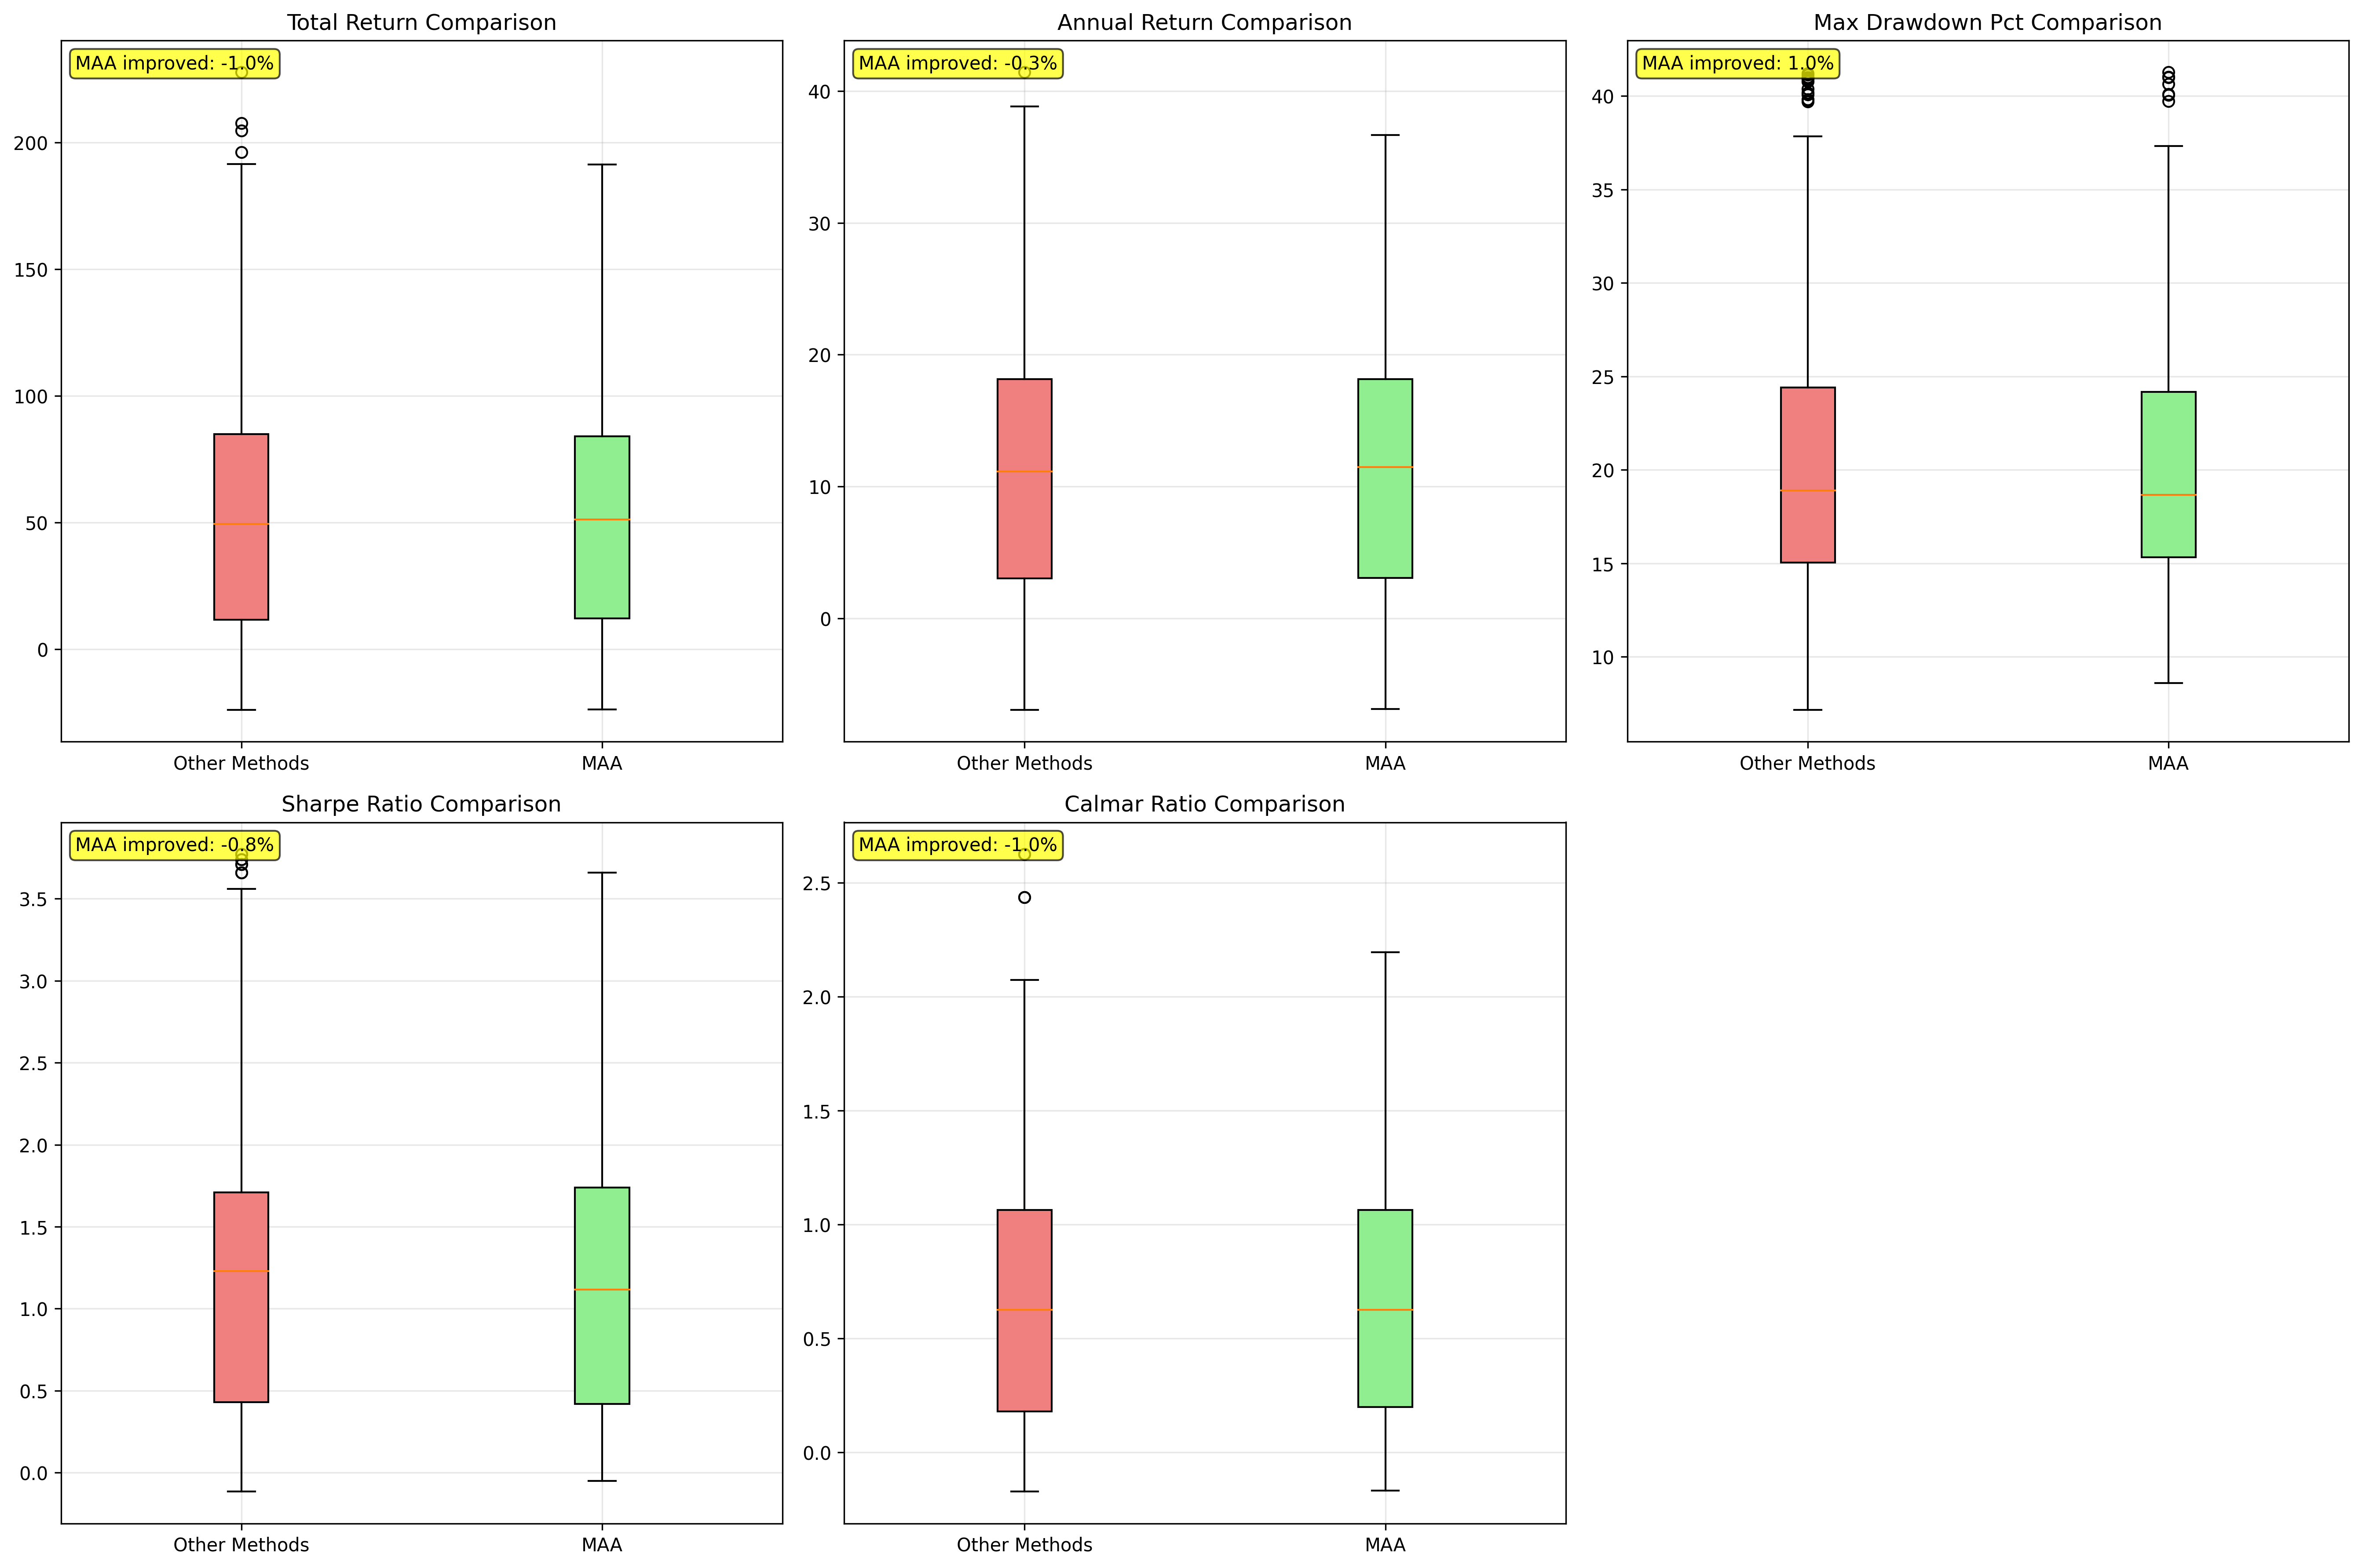
\includegraphics[width=\textwidth]{TongjiThesis-master/data/images/MGCA_vs_Others_Comparison.png}
% \caption{Backtesting comparison of MGCA strategy and other methods on multiple indicators}
% \label{fig:backtest_summary}
% \end{figure*}

% \begin{table*}[h]
% \centering
% \caption{Backtesting performance (investment return, risk, and Sharpe ratio) comparison}
% \label{tab:backtest_metrics}
% \begin{tabular}{lcccc}
% \toprule
% \textbf{Strategy Combination} & \textbf{Total Return} & \textbf{Sharpe} & \textbf{MDD (\%)} & \textbf{Calmar} \\
% \midrule
% Attn Fusion + supervised & \textbf{56.63} & \textbf{1.33} & 20.99 & \textbf{0.72} \\
% Attn Fusion + maa & 50.98 & 1.26 & 21.43 & 0.63 \\
% Gating Fusion + adversarial & 54.40 & 1.25 & 22.27 & 0.60 \\
% Gating Fusion + baseline & 51.07 & 1.24 & 21.20 & 0.64 \\
% \bottomrule
% \end{tabular}
% \end{table*}

% Finally, Table \ref{tab:group_sharpe_best} lists the best Sharpe ratios obtained within different asset groups, further highlighting MGCA's advantage in the "all-group asset" category.

% \begin{table}[h]
% \centering
% \caption{Best Sharpe ratio for each asset group}
% \label{tab:group_sharpe_best}
% \begin{tabular}{lc}
% \toprule
% \textbf{Asset Group} & \textbf{Best Sharpe Ratio} \\
% \midrule
% agriculture & 0.884 \\
% all\_group & \textbf{3.771} \\ 
% base\_metals & 1.739 \\ 
% chemicals & 1.457 \\
% energy & 1.380 \\
% \bottomrule
% \end{tabular}
% \end{table}

% While MGCA may not achieve absolute leading accuracy in all tasks, it consistently demonstrates robust performance across several key metrics, such as the Sharpe ratio and Calmar ratio under Attention Fusion. Notably, it achieves the highest Sharpe ratio (3.771) within the "all-group asset," underscoring MGCA's superior adaptability and generalization capabilities in complex asset structures.

% \begin{figure*}[htbp]
% \centering
% 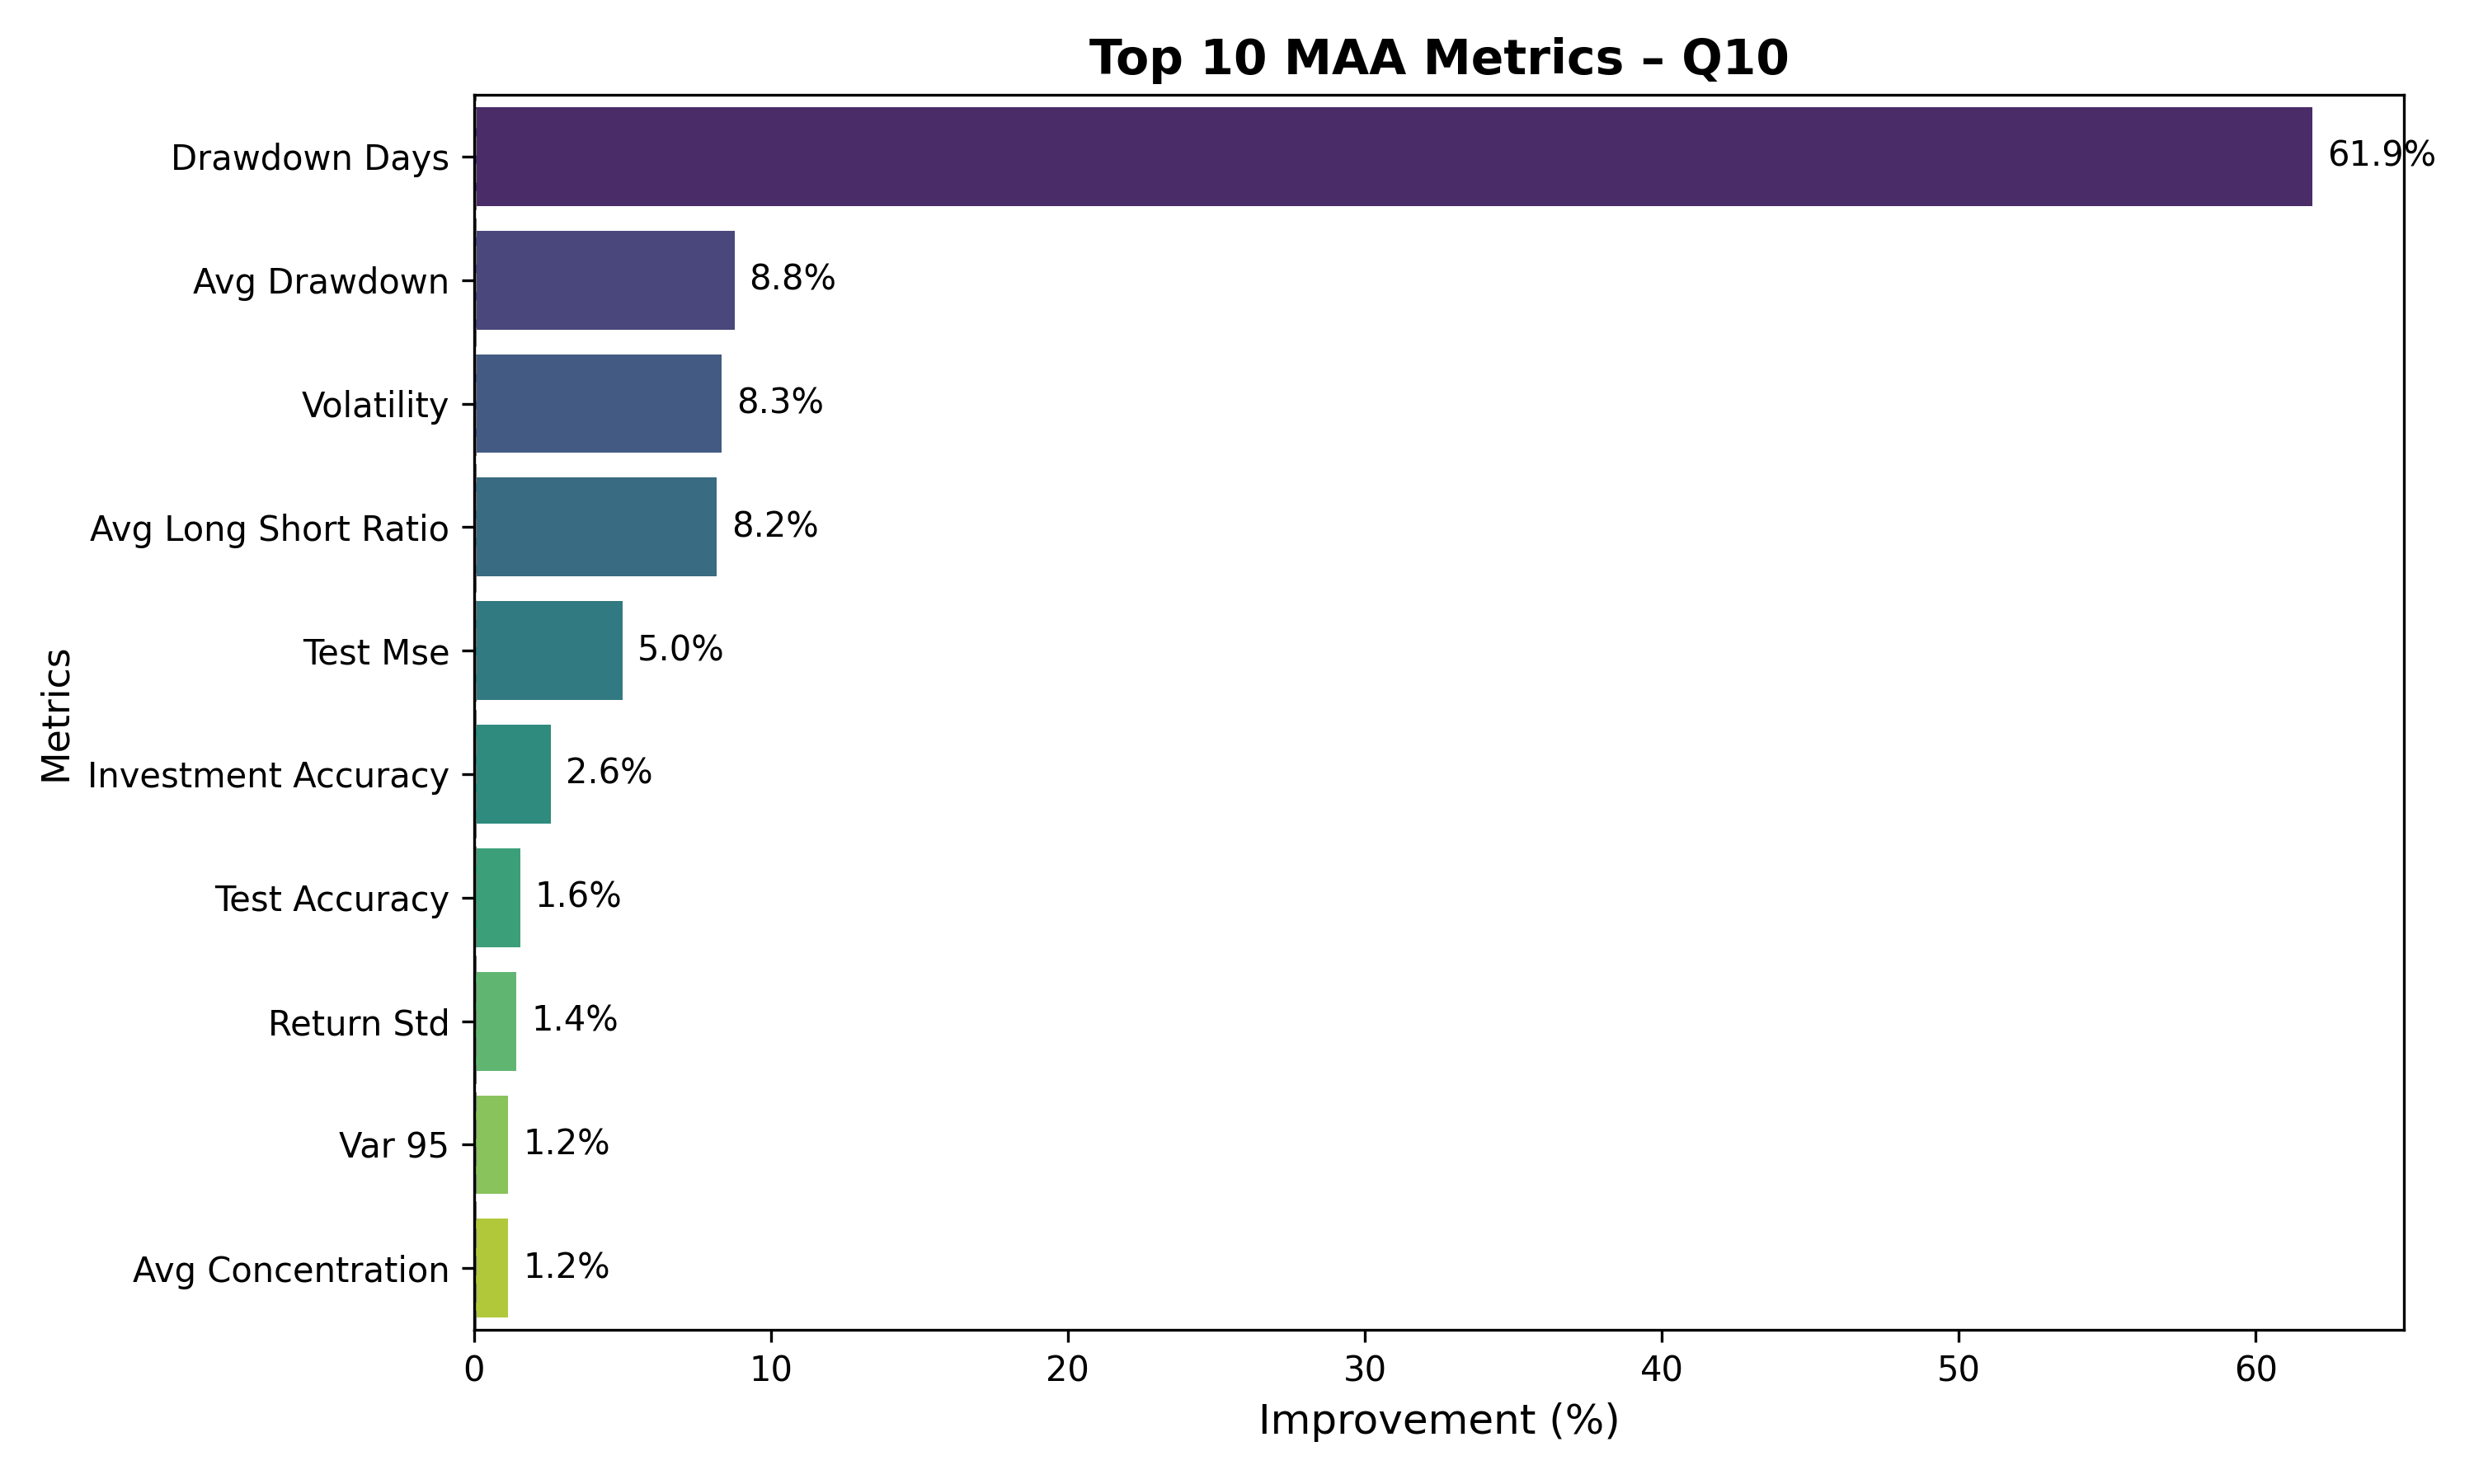
\includegraphics[width=0.48\textwidth]{TongjiThesis-master/data/images/TopN_MGCA_Metrics_Q10.png}
% \hfill
% 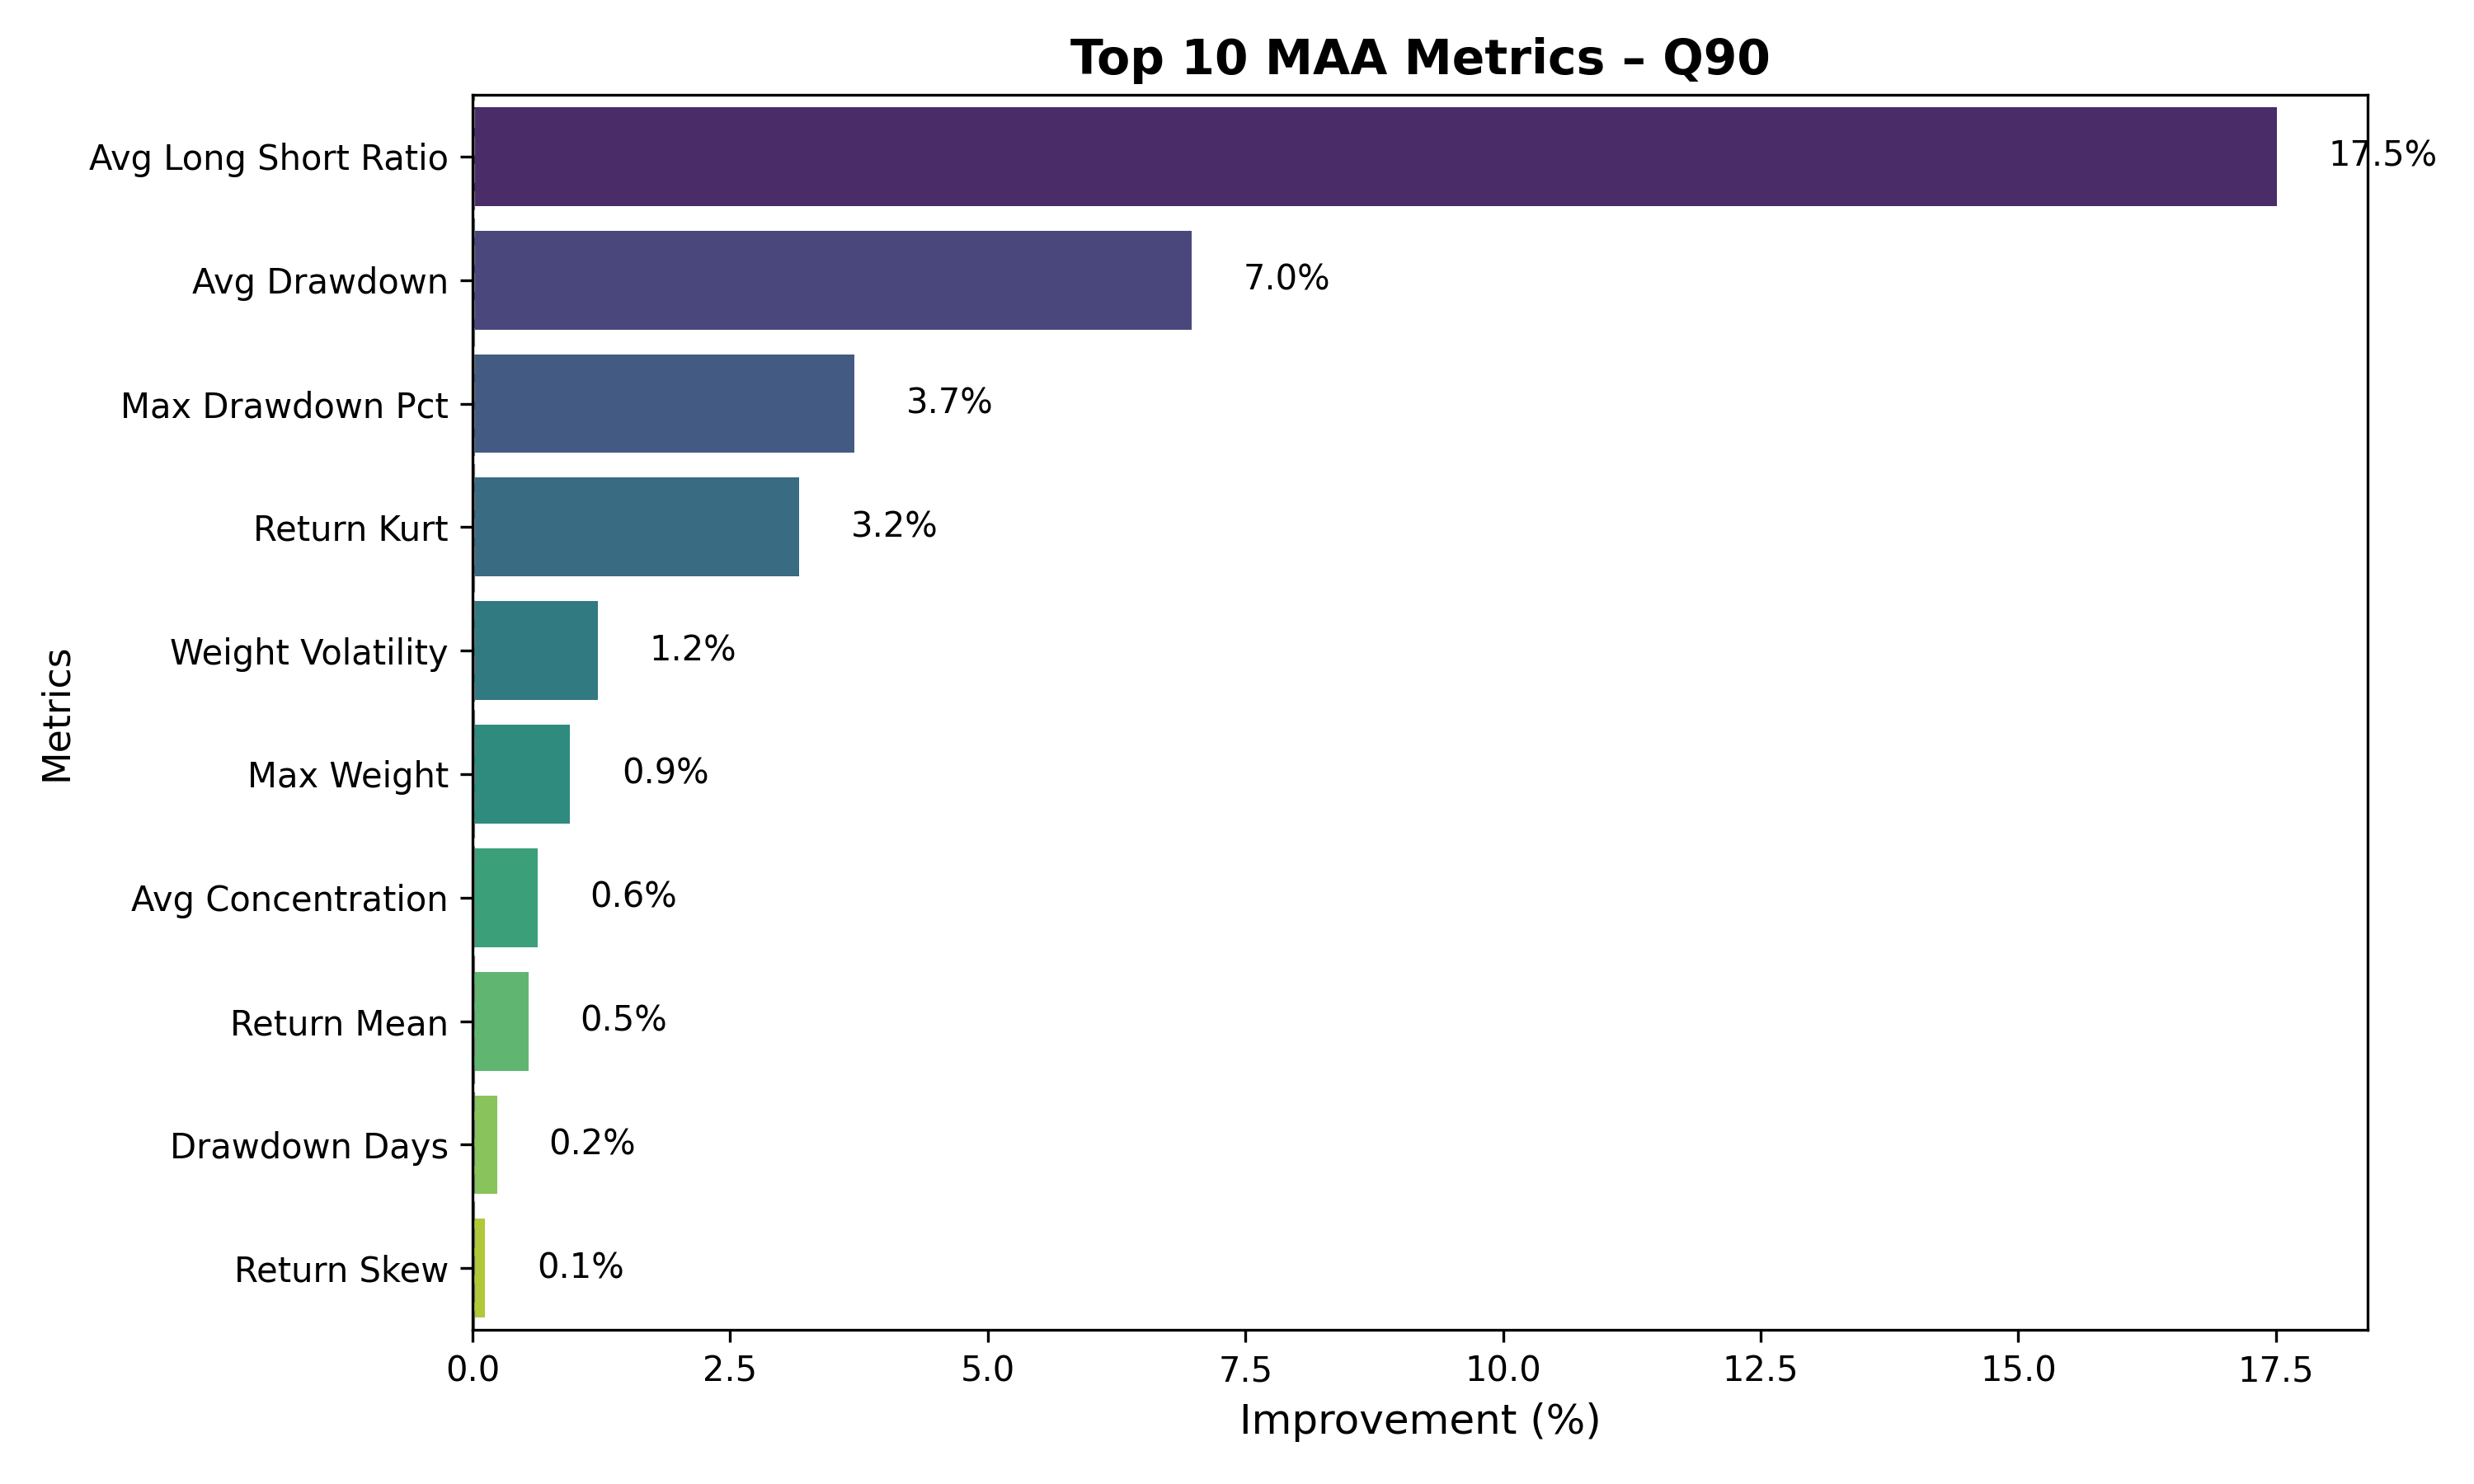
\includegraphics[width=0.48\textwidth]{TongjiThesis-master/data/images/TopN_MGCA_Metrics_Q90.png}
% \caption{MGCA improvement over other pretraining strategies at 10th and 90th percentiles across key metrics}
% \label{fig:topn_q10_q90}
% \end{figure*}

% To further quantify the robustness and high-end potential of the MGCA strategy, we conducted a detailed top-N metric improvement analysis across multiple statistical quantiles. Specifically, we examined the 10th percentile (Q10) and 90th percentile (Q90) improvement percentages of MGCA over other methods across all evaluation metrics. As shown in Figure~\ref{fig:topn_q10_q90}, MGCA exhibits significant improvement in downside risk metrics at the Q10 level—most notably a 61.9\% reduction in \textit{Drawdown Days}, along with notable gains in \textit{Average Drawdown} and \textit{Volatility}, reflecting MGCA’s superior risk control even in worst-case scenarios. Conversely, at the Q90 level, MGCA also demonstrates meaningful advantages in portfolio dynamics and capital efficiency, led by a 17.5\% improvement in \textit{Average Long Short Ratio}, and consistent improvements in \textit{Max Drawdown Percentage} and \textit{Return Kurtosis}. These findings reinforce that MGCA not only performs reliably in adverse market conditions but also scales well in favorable ones, further validating its robustness and flexibility across financial learning tasks.

% In addition to pointwise comparisons, we conducted a comprehensive heatmap analysis to visualize the relative improvement percentages of the MGCA strategy over other pretraining methods across 32 key metrics and 8 statistical percentiles (Min, Q10, Q25, Median, Q75, Q90, Max, Mean) shown in a comprehensive heatmap analysis (Figure \ref{fig:maa_heatmap}). This visualization captures the percentage improvement of MGCA across 32 key financial and behavioral metrics and their corresponding 8 statistical percentiles (Min, Q10, Q25, Median, Q75, Q90, Max, Mean).

% \begin{figure*}[htbp]
% \centering
% 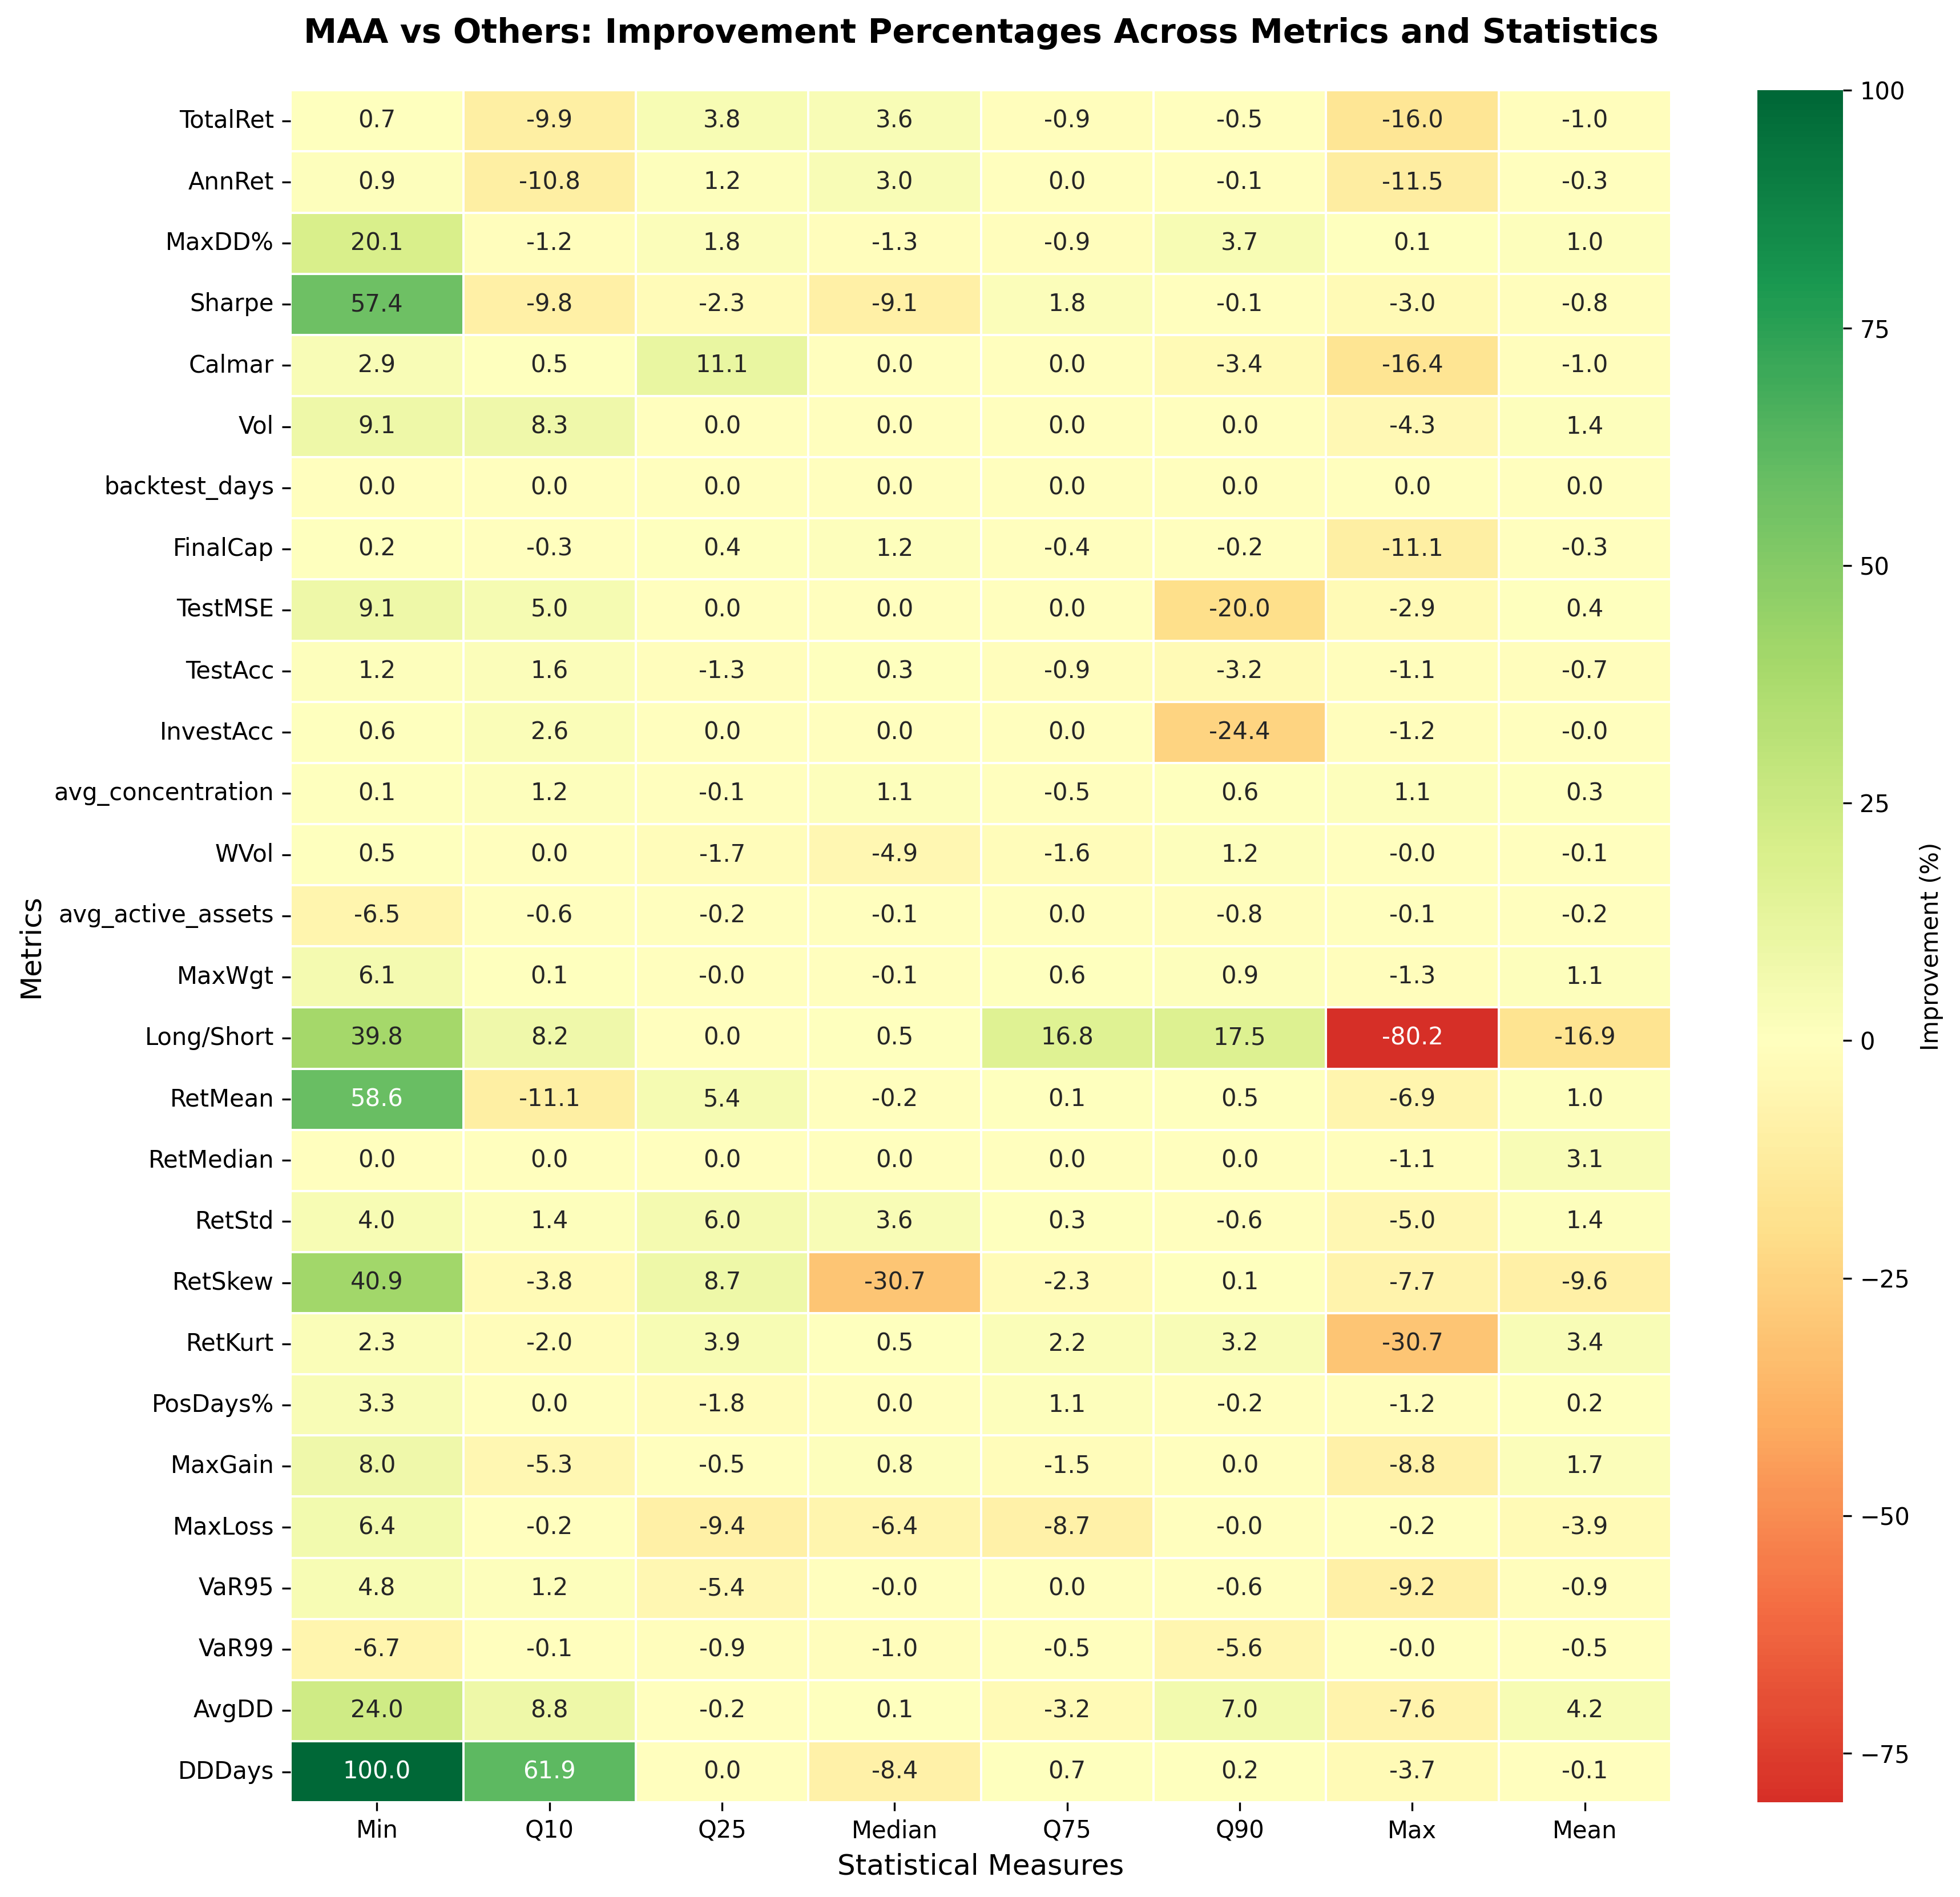
\includegraphics[width=0.95\textwidth]{TongjiThesis-master/data/images/MGCA_vs_Others_Heatmap.png}
% \caption{Heatmap of MGCA improvement percentages across 32 metrics and 8 statistical percentiles compared to other pretraining methods}
% \label{fig:maa_heatmap}
% \end{figure*}

% From the heatmap analysis across various statistical quantiles (Min, Q10, Median, Q90, Max), it is evident that the MGCA strategy does not dominate across all metrics or quantiles, but demonstrates relative advantages in different dimensions depending on the statistical measure applied. Specifically, when metrics are sorted and examined at lower quantiles (e.g., Q10 or Q25), MGCA consistently outperforms other methods in risk-related dimensions such as Drawdown Days, Average Drawdown, and Volatility. This suggests a robustness advantage under worst-case or conservative scenarios.

% The heatmap distinctly highlights MGCA's consistent and substantial enhancements across multiple performance dimensions, particularly in risk management and capital preservation. A compelling example is Drawdown Days (DDDays), which demonstrates an exceptional 100.0\% improvement at the minimum percentile, signifying MGCA's unparalleled capacity to entirely mitigate the longest drawdown periods observed in baseline methods. This robust performance extends to 61.9\% improvement at the 10th percentile (Q10) and sustains significant advantages across most quantiles, unequivocally underscoring MGCA's superior resilience in adverse market conditions. Similarly, metrics such as Average Drawdown (AvgDD) (e.g., 8.8\% at Q10) and Volatility (Vol) (e.g., 9.1\% at Min, 8.3\% at Q10) consistently exhibit positive improvements within their lower quantiles, further validating MGCA's ability to enhance risk control and portfolio stability. Notably, the Sharpe Ratio also shows a remarkable 57.4\% improvement at its minimum percentile, indicating MGCA's strong potential for superior risk-adjusted returns even under less favorable market conditions.

% Interestingly, this pattern implies that the MGCA strategy may embed certain implicit hedging capabilities, where in more conservative market environments, it achieves either stable gains or reduced losses compared to its peers. While it may not maximize performance at upper extremes (as seen in Q90 or Max for some indicators), its ability to maintain solid performance at the lower end highlights its utility for risk-averse portfolio management or in volatile conditions.

% Furthermore, MGCA demonstrates notable improvements for specific metrics critical to tactical asset allocation and the characteristics of return distributions. For instance, the Average Long Short Ratio (Long/Short) exhibits positive improvements at Q75 (16.8\%) and Q90 (17.5\%), suggesting an enhanced ability to express directional conviction and optimize exposure in typical to favorable market conditions. Similarly, Return Skewness (RetSkew) shows a significant 40.9\% improvement at its minimum percentile, indicating a more favorable left-tail behavior of returns. The Return Mean (RetMean) also sees a substantial 58.6\% improvement at its minimum percentile. These gains collectively suggest MGCA's capacity to refine overall return profiles and manage exposure effectively.

% Overall, MGCA demonstrates non-uniform but strategically distributed improvements, indicating that it adapts better under specific market stress conditions rather than universally outperforming in all scenarios.

% While the overall trend robustly underscores MGCA's outperformance, a nuanced examination of the heatmap also identifies specific areas for further refinement and investigation. Certain metrics, such as Annual Return (AnnRet) (e.g., -11.5\% at Max), Test MSE (e.g., -20.0\% at Q75), and Investment Accuracy (InvestAcc) (e.g., -24.4\% at Q90), exhibit localized negative improvements at higher quantiles. These observations do not necessarily imply fundamental flaws but rather suggest a potential for over-optimization or an accentuated response to specific market regimes under highly favorable conditions, where MGCA's adaptive positioning might lead to larger deviations from the baseline. Similarly, while the Sharpe Ratio shows a strong minimum improvement, it exhibits negative improvements across several other quantiles, indicating that while MGCA can achieve high risk-adjusted returns in worst-case scenarios, its average or typical performance in this regard might warrant further tuning. These insights highlight the importance of calibrating MGCA's deployment within real-world trading systems, ensuring its benefits are maximized while considering its sensitivity to extreme positive scenarios. Such findings guide future research towards dynamic adaptation mechanisms for MGCA, further solidifying its robust performance profile.

% \subsection{MGCA with Highest Return}\label{sec:appendix MGCA_high_return}
% The return distribution plot reveals a slight positive skew, with positive returns dominating, indicating a clear profitability bias and effective tail risk control with limited extreme negative return events. This distributional characteristic further supports why its Sharpe ratio remained robust even in a high-return environment.

% \begin{figure*}[h]
% \centering
% 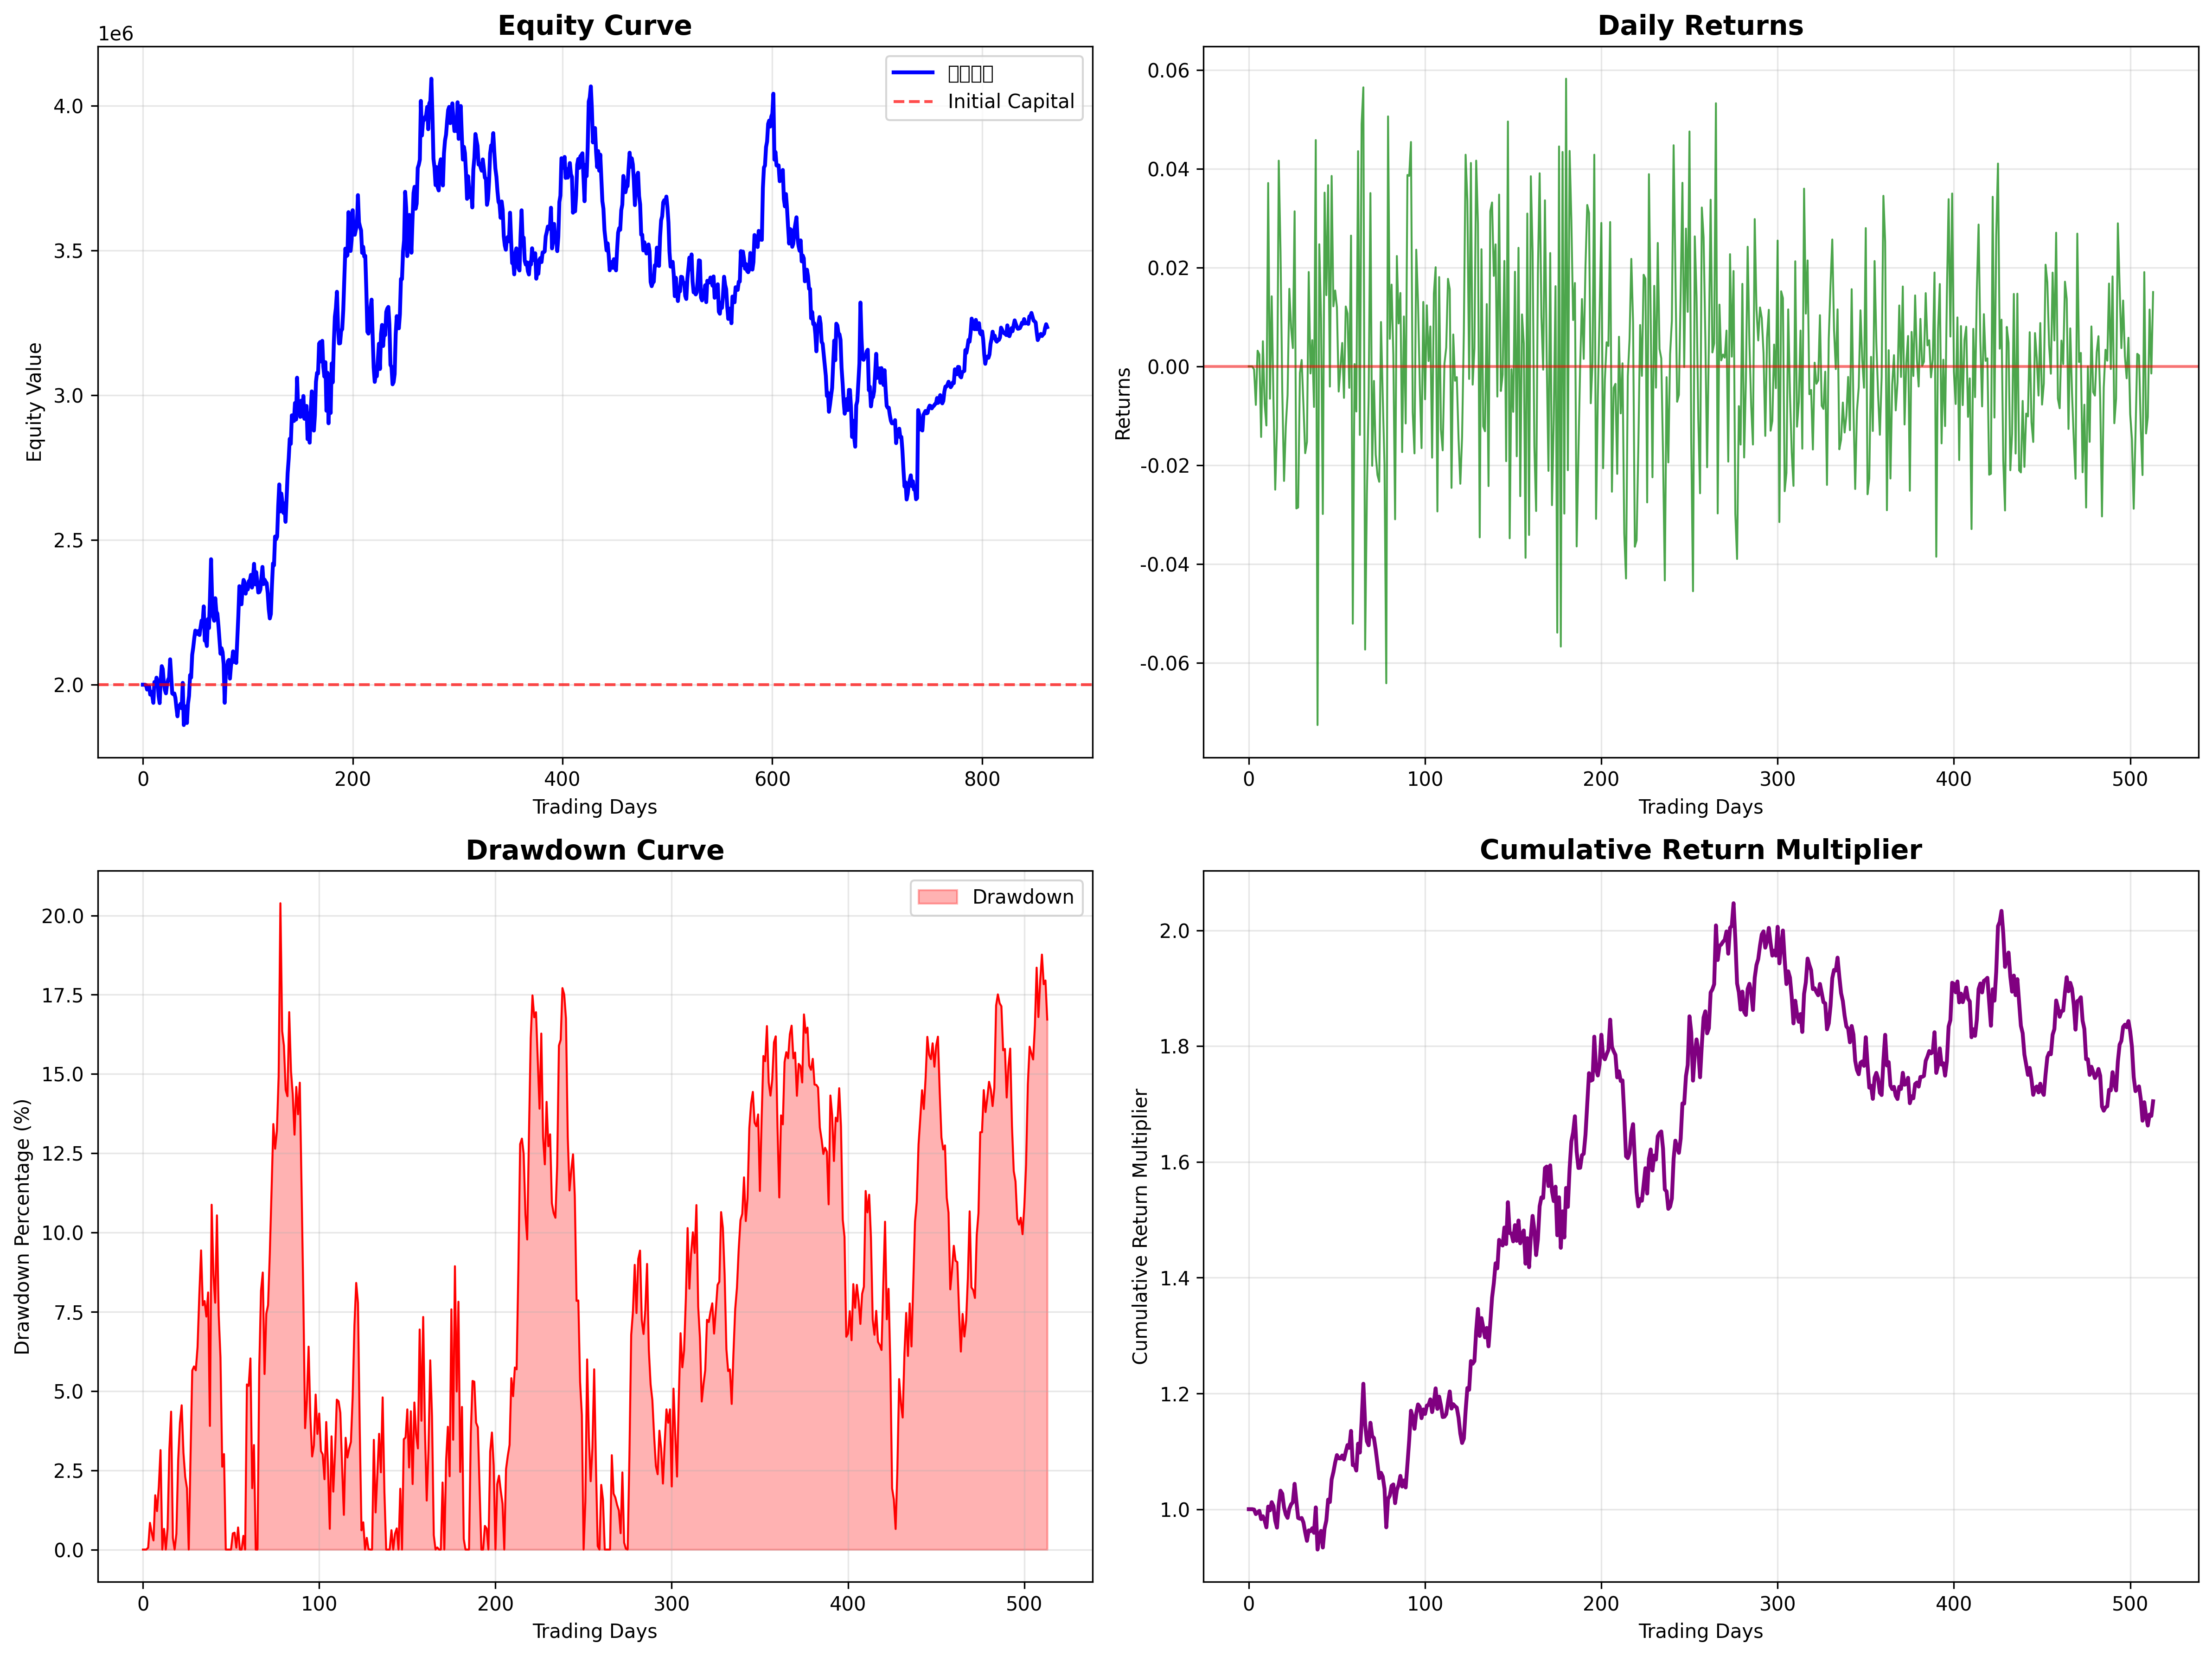
\includegraphics[width=\textwidth]{TongjiThesis-master/data/images/comprehensive_performance_concat_MGC_3assets.png}
% \caption{Dynamic asset allocation weights of MGCA strategy under chemicals asset group}
% \label{fig:highest_return_weights}
% \end{figure*}

% Additionally, Figure \ref{fig:highest_return_weights} depicts the dynamic asset allocation weights of this strategy during its operation. The strategy achieved stable yet flexible position adjustments across the three chemical assets, highlighting the MGCA framework's powerful ability to learn structural features among assets.

% Specifically, PTA held an average weight of -0.4471, indicating a consistent short position, suggesting the strategy accurately identified its downward trend. PVC maintained an average weight of 0.3507, serving as the primary long asset and steadily contributing positive returns. PP exhibited the least weight fluctuation, averaging approximately 0.0962, playing an auxiliary long role.

% In conclusion, the MGCA strategy under this configuration effectively managed risk while achieving substantial return growth through flexible position scheduling and efficient learning of asset structures. This capability fully demonstrates MGCA's high return potential and practical value in multi-asset quantitative modeling.











